% Feature Selection Chapter
% This chapter assumes the following directory structure:
% report/
%   ├── feature_selection.tex (this file)
%   ├── figures/              (correlation matrices and pairplots)
%   └── logs/                 (TopFeaturesTable.tex, FeatureSelectionCommands.tex, and other outputs)
%
% Run the Python feature selection script first to generate all required files

% Include the automatically generated commands
% Feature Selection LaTeX Commands - iBudget
% Generated: 2025-10-09 20:25:43
% Include with: % Feature Selection LaTeX Commands - iBudget
% Generated: 2025-10-09 20:25:43
% Include with: % Feature Selection LaTeX Commands - iBudget
% Generated: 2025-10-09 20:25:43
% Include with: \input{report/logs/FeatureSelectionCommands.tex}

\newcommand{\FSNumFiscalYears}{6}

% Methodological note
\newcommand{\FSNoteMI}{Mutual information is not on a universal scale across years; consider z-scoring per year before averaging.}

% Dataset sizes
\newcommand{\FSMinRecordsTotal}{42,677}
\newcommand{\FSMaxRecordsTotal}{47,797}
\newcommand{\FSMeanRecordsTotal}{45,527}

\newcommand{\FSMinRecordsFiltered}{41,570}
\newcommand{\FSMaxRecordsFiltered}{47,337}

\newcommand{\FSMinRecordsFinal}{29,566}
\newcommand{\FSMaxRecordsFinal}{35,329}

% Feature counts
\newcommand{\FSNumCandidateVariables}{52}
\newcommand{\FSFeaturesAllYears}{8}
\newcommand{\FSFeaturesMostYears}{9}

% FY2025
\newcommand{\FSRecordsTotalFYTwoThousandTwentyFive}{47,797}
\newcommand{\FSRecordsFilteredFYTwoThousandTwentyFive}{47,337}
\newcommand{\FSRecordsFinalFYTwoThousandTwentyFive}{35,329}
\newcommand{\FSTopFeatureFYTwoThousandTwentyFive}{RESIDENCETYPE}
\newcommand{\FSTopMIFYTwoThousandTwentyFive}{0.3237}

% FY2024
\newcommand{\FSRecordsTotalFYTwoThousandTwentyFour}{47,259}
\newcommand{\FSRecordsFilteredFYTwoThousandTwentyFour}{46,269}
\newcommand{\FSRecordsFinalFYTwoThousandTwentyFour}{34,034}
\newcommand{\FSTopFeatureFYTwoThousandTwentyFour}{RESIDENCETYPE}
\newcommand{\FSTopMIFYTwoThousandTwentyFour}{0.3184}

% FY2023
\newcommand{\FSRecordsTotalFYTwoThousandTwentyThree}{46,193}
\newcommand{\FSRecordsFilteredFYTwoThousandTwentyThree}{45,359}
\newcommand{\FSRecordsFinalFYTwoThousandTwentyThree}{33,001}
\newcommand{\FSTopFeatureFYTwoThousandTwentyThree}{RESIDENCETYPE}
\newcommand{\FSTopMIFYTwoThousandTwentyThree}{0.3129}

% FY2022
\newcommand{\FSRecordsTotalFYTwoThousandTwentyTwo}{45,270}
\newcommand{\FSRecordsFilteredFYTwoThousandTwentyTwo}{44,090}
\newcommand{\FSRecordsFinalFYTwoThousandTwentyTwo}{32,107}
\newcommand{\FSTopFeatureFYTwoThousandTwentyTwo}{RESIDENCETYPE}
\newcommand{\FSTopMIFYTwoThousandTwentyTwo}{0.3185}

% FY2021
\newcommand{\FSRecordsTotalFYTwoThousandTwentyOne}{43,968}
\newcommand{\FSRecordsFilteredFYTwoThousandTwentyOne}{42,779}
\newcommand{\FSRecordsFinalFYTwoThousandTwentyOne}{30,738}
\newcommand{\FSTopFeatureFYTwoThousandTwentyOne}{RESIDENCETYPE}
\newcommand{\FSTopMIFYTwoThousandTwentyOne}{0.3102}

% FY2020
\newcommand{\FSRecordsTotalFYTwoThousandTwenty}{42,677}
\newcommand{\FSRecordsFilteredFYTwoThousandTwenty}{41,570}
\newcommand{\FSRecordsFinalFYTwoThousandTwenty}{29,566}
\newcommand{\FSTopFeatureFYTwoThousandTwenty}{RESIDENCETYPE}
\newcommand{\FSTopMIFYTwoThousandTwenty}{0.3146}



\newcommand{\FSNumFiscalYears}{6}

% Methodological note
\newcommand{\FSNoteMI}{Mutual information is not on a universal scale across years; consider z-scoring per year before averaging.}

% Dataset sizes
\newcommand{\FSMinRecordsTotal}{42,677}
\newcommand{\FSMaxRecordsTotal}{47,797}
\newcommand{\FSMeanRecordsTotal}{45,527}

\newcommand{\FSMinRecordsFiltered}{41,570}
\newcommand{\FSMaxRecordsFiltered}{47,337}

\newcommand{\FSMinRecordsFinal}{29,566}
\newcommand{\FSMaxRecordsFinal}{35,329}

% Feature counts
\newcommand{\FSNumCandidateVariables}{52}
\newcommand{\FSFeaturesAllYears}{8}
\newcommand{\FSFeaturesMostYears}{9}

% FY2025
\newcommand{\FSRecordsTotalFYTwoThousandTwentyFive}{47,797}
\newcommand{\FSRecordsFilteredFYTwoThousandTwentyFive}{47,337}
\newcommand{\FSRecordsFinalFYTwoThousandTwentyFive}{35,329}
\newcommand{\FSTopFeatureFYTwoThousandTwentyFive}{RESIDENCETYPE}
\newcommand{\FSTopMIFYTwoThousandTwentyFive}{0.3237}

% FY2024
\newcommand{\FSRecordsTotalFYTwoThousandTwentyFour}{47,259}
\newcommand{\FSRecordsFilteredFYTwoThousandTwentyFour}{46,269}
\newcommand{\FSRecordsFinalFYTwoThousandTwentyFour}{34,034}
\newcommand{\FSTopFeatureFYTwoThousandTwentyFour}{RESIDENCETYPE}
\newcommand{\FSTopMIFYTwoThousandTwentyFour}{0.3184}

% FY2023
\newcommand{\FSRecordsTotalFYTwoThousandTwentyThree}{46,193}
\newcommand{\FSRecordsFilteredFYTwoThousandTwentyThree}{45,359}
\newcommand{\FSRecordsFinalFYTwoThousandTwentyThree}{33,001}
\newcommand{\FSTopFeatureFYTwoThousandTwentyThree}{RESIDENCETYPE}
\newcommand{\FSTopMIFYTwoThousandTwentyThree}{0.3129}

% FY2022
\newcommand{\FSRecordsTotalFYTwoThousandTwentyTwo}{45,270}
\newcommand{\FSRecordsFilteredFYTwoThousandTwentyTwo}{44,090}
\newcommand{\FSRecordsFinalFYTwoThousandTwentyTwo}{32,107}
\newcommand{\FSTopFeatureFYTwoThousandTwentyTwo}{RESIDENCETYPE}
\newcommand{\FSTopMIFYTwoThousandTwentyTwo}{0.3185}

% FY2021
\newcommand{\FSRecordsTotalFYTwoThousandTwentyOne}{43,968}
\newcommand{\FSRecordsFilteredFYTwoThousandTwentyOne}{42,779}
\newcommand{\FSRecordsFinalFYTwoThousandTwentyOne}{30,738}
\newcommand{\FSTopFeatureFYTwoThousandTwentyOne}{RESIDENCETYPE}
\newcommand{\FSTopMIFYTwoThousandTwentyOne}{0.3102}

% FY2020
\newcommand{\FSRecordsTotalFYTwoThousandTwenty}{42,677}
\newcommand{\FSRecordsFilteredFYTwoThousandTwenty}{41,570}
\newcommand{\FSRecordsFinalFYTwoThousandTwenty}{29,566}
\newcommand{\FSTopFeatureFYTwoThousandTwenty}{RESIDENCETYPE}
\newcommand{\FSTopMIFYTwoThousandTwenty}{0.3146}



\newcommand{\FSNumFiscalYears}{6}

% Methodological note
\newcommand{\FSNoteMI}{Mutual information is not on a universal scale across years; consider z-scoring per year before averaging.}

% Dataset sizes
\newcommand{\FSMinRecordsTotal}{42,677}
\newcommand{\FSMaxRecordsTotal}{47,797}
\newcommand{\FSMeanRecordsTotal}{45,527}

\newcommand{\FSMinRecordsFiltered}{41,570}
\newcommand{\FSMaxRecordsFiltered}{47,337}

\newcommand{\FSMinRecordsFinal}{29,566}
\newcommand{\FSMaxRecordsFinal}{35,329}

% Feature counts
\newcommand{\FSNumCandidateVariables}{52}
\newcommand{\FSFeaturesAllYears}{8}
\newcommand{\FSFeaturesMostYears}{9}

% FY2025
\newcommand{\FSRecordsTotalFYTwoThousandTwentyFive}{47,797}
\newcommand{\FSRecordsFilteredFYTwoThousandTwentyFive}{47,337}
\newcommand{\FSRecordsFinalFYTwoThousandTwentyFive}{35,329}
\newcommand{\FSTopFeatureFYTwoThousandTwentyFive}{RESIDENCETYPE}
\newcommand{\FSTopMIFYTwoThousandTwentyFive}{0.3237}

% FY2024
\newcommand{\FSRecordsTotalFYTwoThousandTwentyFour}{47,259}
\newcommand{\FSRecordsFilteredFYTwoThousandTwentyFour}{46,269}
\newcommand{\FSRecordsFinalFYTwoThousandTwentyFour}{34,034}
\newcommand{\FSTopFeatureFYTwoThousandTwentyFour}{RESIDENCETYPE}
\newcommand{\FSTopMIFYTwoThousandTwentyFour}{0.3184}

% FY2023
\newcommand{\FSRecordsTotalFYTwoThousandTwentyThree}{46,193}
\newcommand{\FSRecordsFilteredFYTwoThousandTwentyThree}{45,359}
\newcommand{\FSRecordsFinalFYTwoThousandTwentyThree}{33,001}
\newcommand{\FSTopFeatureFYTwoThousandTwentyThree}{RESIDENCETYPE}
\newcommand{\FSTopMIFYTwoThousandTwentyThree}{0.3129}

% FY2022
\newcommand{\FSRecordsTotalFYTwoThousandTwentyTwo}{45,270}
\newcommand{\FSRecordsFilteredFYTwoThousandTwentyTwo}{44,090}
\newcommand{\FSRecordsFinalFYTwoThousandTwentyTwo}{32,107}
\newcommand{\FSTopFeatureFYTwoThousandTwentyTwo}{RESIDENCETYPE}
\newcommand{\FSTopMIFYTwoThousandTwentyTwo}{0.3185}

% FY2021
\newcommand{\FSRecordsTotalFYTwoThousandTwentyOne}{43,968}
\newcommand{\FSRecordsFilteredFYTwoThousandTwentyOne}{42,779}
\newcommand{\FSRecordsFinalFYTwoThousandTwentyOne}{30,738}
\newcommand{\FSTopFeatureFYTwoThousandTwentyOne}{RESIDENCETYPE}
\newcommand{\FSTopMIFYTwoThousandTwentyOne}{0.3102}

% FY2020
\newcommand{\FSRecordsTotalFYTwoThousandTwenty}{42,677}
\newcommand{\FSRecordsFilteredFYTwoThousandTwenty}{41,570}
\newcommand{\FSRecordsFinalFYTwoThousandTwenty}{29,566}
\newcommand{\FSTopFeatureFYTwoThousandTwenty}{RESIDENCETYPE}
\newcommand{\FSTopMIFYTwoThousandTwenty}{0.3146}



\chapter{Feature Selection}
\label{ch:feature-selection}

\section{Introduction}
\label{sec:feature-selection-intro}

The selection of appropriate predictive features constitutes a critical component in developing robust cost prediction models for the Florida Agency for Persons with Disabilities (APD) iBudget algorithm. This chapter presents a comprehensive methodology for identifying and evaluating candidate variables through a multi-faceted approach combining information-theoretic measures, correlation analysis, visual inspection techniques, and domain expertise. The systematic feature selection process aims to maximize predictive accuracy while maintaining model interpretability and computational efficiency.

\section{Methodology}
\label{sec:feature-selection-methodology}

\subsection{Data Preparation and Quality Filtering}
\label{subsec:data-preparation}

Prior to feature selection analysis, stringent data quality filters were applied to ensure the reliability of statistical metrics. Records were included only when satisfying the following criteria:
\begin{itemize}
    \item \texttt{LateEntry} = 0
    \item \texttt{EarlyExit} = 0
    \item \texttt{MissingQSI} = 0
    \item \texttt{InsufficientDays} = 0
\end{itemize}

These filters ensured that all analyzed records contained complete Quality Service Indicator (QSI) assessments and represented full fiscal year service utilization patterns. The filtering process reduced the initial dataset from approximately \FSMinRecordsTotal{} to \FSMaxRecordsTotal{} total records per fiscal year to between \FSMinRecordsFinal{} and \FSMaxRecordsFinal{} high-quality records suitable for statistical analysis.

\subsection{Mutual Information Analysis}
\label{subsec:mutual-information}

Mutual information (MI) was employed as the primary metric for quantifying statistical dependencies between candidate features and the target variable (\texttt{TotalCost}). Unlike correlation coefficients, MI captures both linear and non-linear relationships without assuming any particular functional form. For continuous variables $X$ and $Y$, mutual information is defined as:

\begin{equation}
I(X;Y) = \int\int p(x,y) \log\left(\frac{p(x,y)}{p(x)p(y)}\right) dx\,dy
\label{eq:mutual-information}
\end{equation}

where $p(x,y)$ represents the joint probability density function and $p(x)$, $p(y)$ denote the marginal densities. MI values range from 0 (indicating independence) to positive values indicating increasing dependency strength.

The mutual information scores were calculated between each of the \FSNumCandidateVariables{} candidate variables and \texttt{TotalCost} using the scikit-learn implementation with automatic discretization for continuous variables. Features were subsequently ranked by their MI scores to identify the most informative predictors.

\subsection{Correlation Analysis for Multicollinearity Detection}
\label{subsec:correlation-analysis}

To identify and manage multicollinearity among predictor variables, Spearman rank correlation matrices were computed for all feature pairs. Spearman correlation was selected over Pearson correlation to accommodate non-linear monotonic relationships and to be robust against outliers. The Spearman correlation coefficient $\rho$ between variables $X$ and $Y$ is computed as:
%
\begin{equation}
\rho = 1 - \frac{6\sum_{i=1}^{n}d_i^2}{n(n^2-1)}
\label{eq:spearman}
\end{equation}
%
where $d_i$ represents the difference between ranks of corresponding values and $n$ denotes the sample size.

A threshold of $|\rho| > \FSCorrelationThreshold$ was established to identify highly correlated feature pairs. When such pairs were detected, the feature with higher mutual information with the target variable was retained, while the redundant feature was marked for potential exclusion to reduce multicollinearity and improve model interpretability.

\subsection{Visual Relationship Assessment}
\label{subsec:visual-assessment}

Pairwise scatter plot matrices were generated for the top-ranked features to visually inspect:
\begin{enumerate}
    \item The functional form of relationships between predictors and the target
    \item The presence of non-linear patterns not captured by correlation coefficients
    \item Outlier observations requiring special consideration
    \item Natural clustering patterns in the feature space
    \item Heteroscedasticity patterns affecting model assumptions
\end{enumerate}

These visualizations complemented the quantitative metrics by revealing complex interaction patterns and data quality issues not apparent from summary statistics alone.

\subsection{Domain Knowledge Integration}
\label{subsec:domain-knowledge}

Statistical metrics were augmented with regulatory requirements and clinical expertise to ensure selected features aligned with policy objectives and clinical validity. Specifically:

\begin{itemize}
    \item Variables mandated by Florida Administrative Code or federal regulations were included regardless of statistical significance
    \item Clinical assessment scores (QSI questions Q\FSQSIFunctionalStart--Q\FSQSIFunctionalEnd, Q\FSQSIBehavioralStart--Q\FSQSIBehavioralEnd, Q\FSQSIPhysicalStart--Q\FSQSIPhysicalEnd) were retained as complete subscales to maintain instrument validity
    \item Demographic variables (\texttt{Age}, \texttt{Gender}, \texttt{Race}, \texttt{Ethnicity}) were preserved to enable equity analyses
    \item Service setting variables (\texttt{RESIDENCETYPE}, \texttt{LivingSetting}) were prioritized given their established relationship with care intensity
\end{itemize}

\section{Results by Fiscal Year}
\label{sec:results-by-year}

\subsection{Fiscal Year 2020}
\label{subsec:fy2020}

Analysis of FY2020 data (n=\FSRecordsFinalFYTwoThousandTwenty) revealed \FSTopFeatureFYTwoThousandTwenty{} as the dominant predictor with MI=\FSTopMIFYTwoThousandTwenty, followed by additional key predictors. The correlation analysis identified strong relationships among the summary scores and their component levels, with Spearman correlations exceeding \FSCorrelationThreshold{} for pairs such as \texttt{BSum}--\texttt{BLEVEL} and \texttt{FSum}--\texttt{FLEVEL}.

\begin{figure}[htbp]
    \centering
    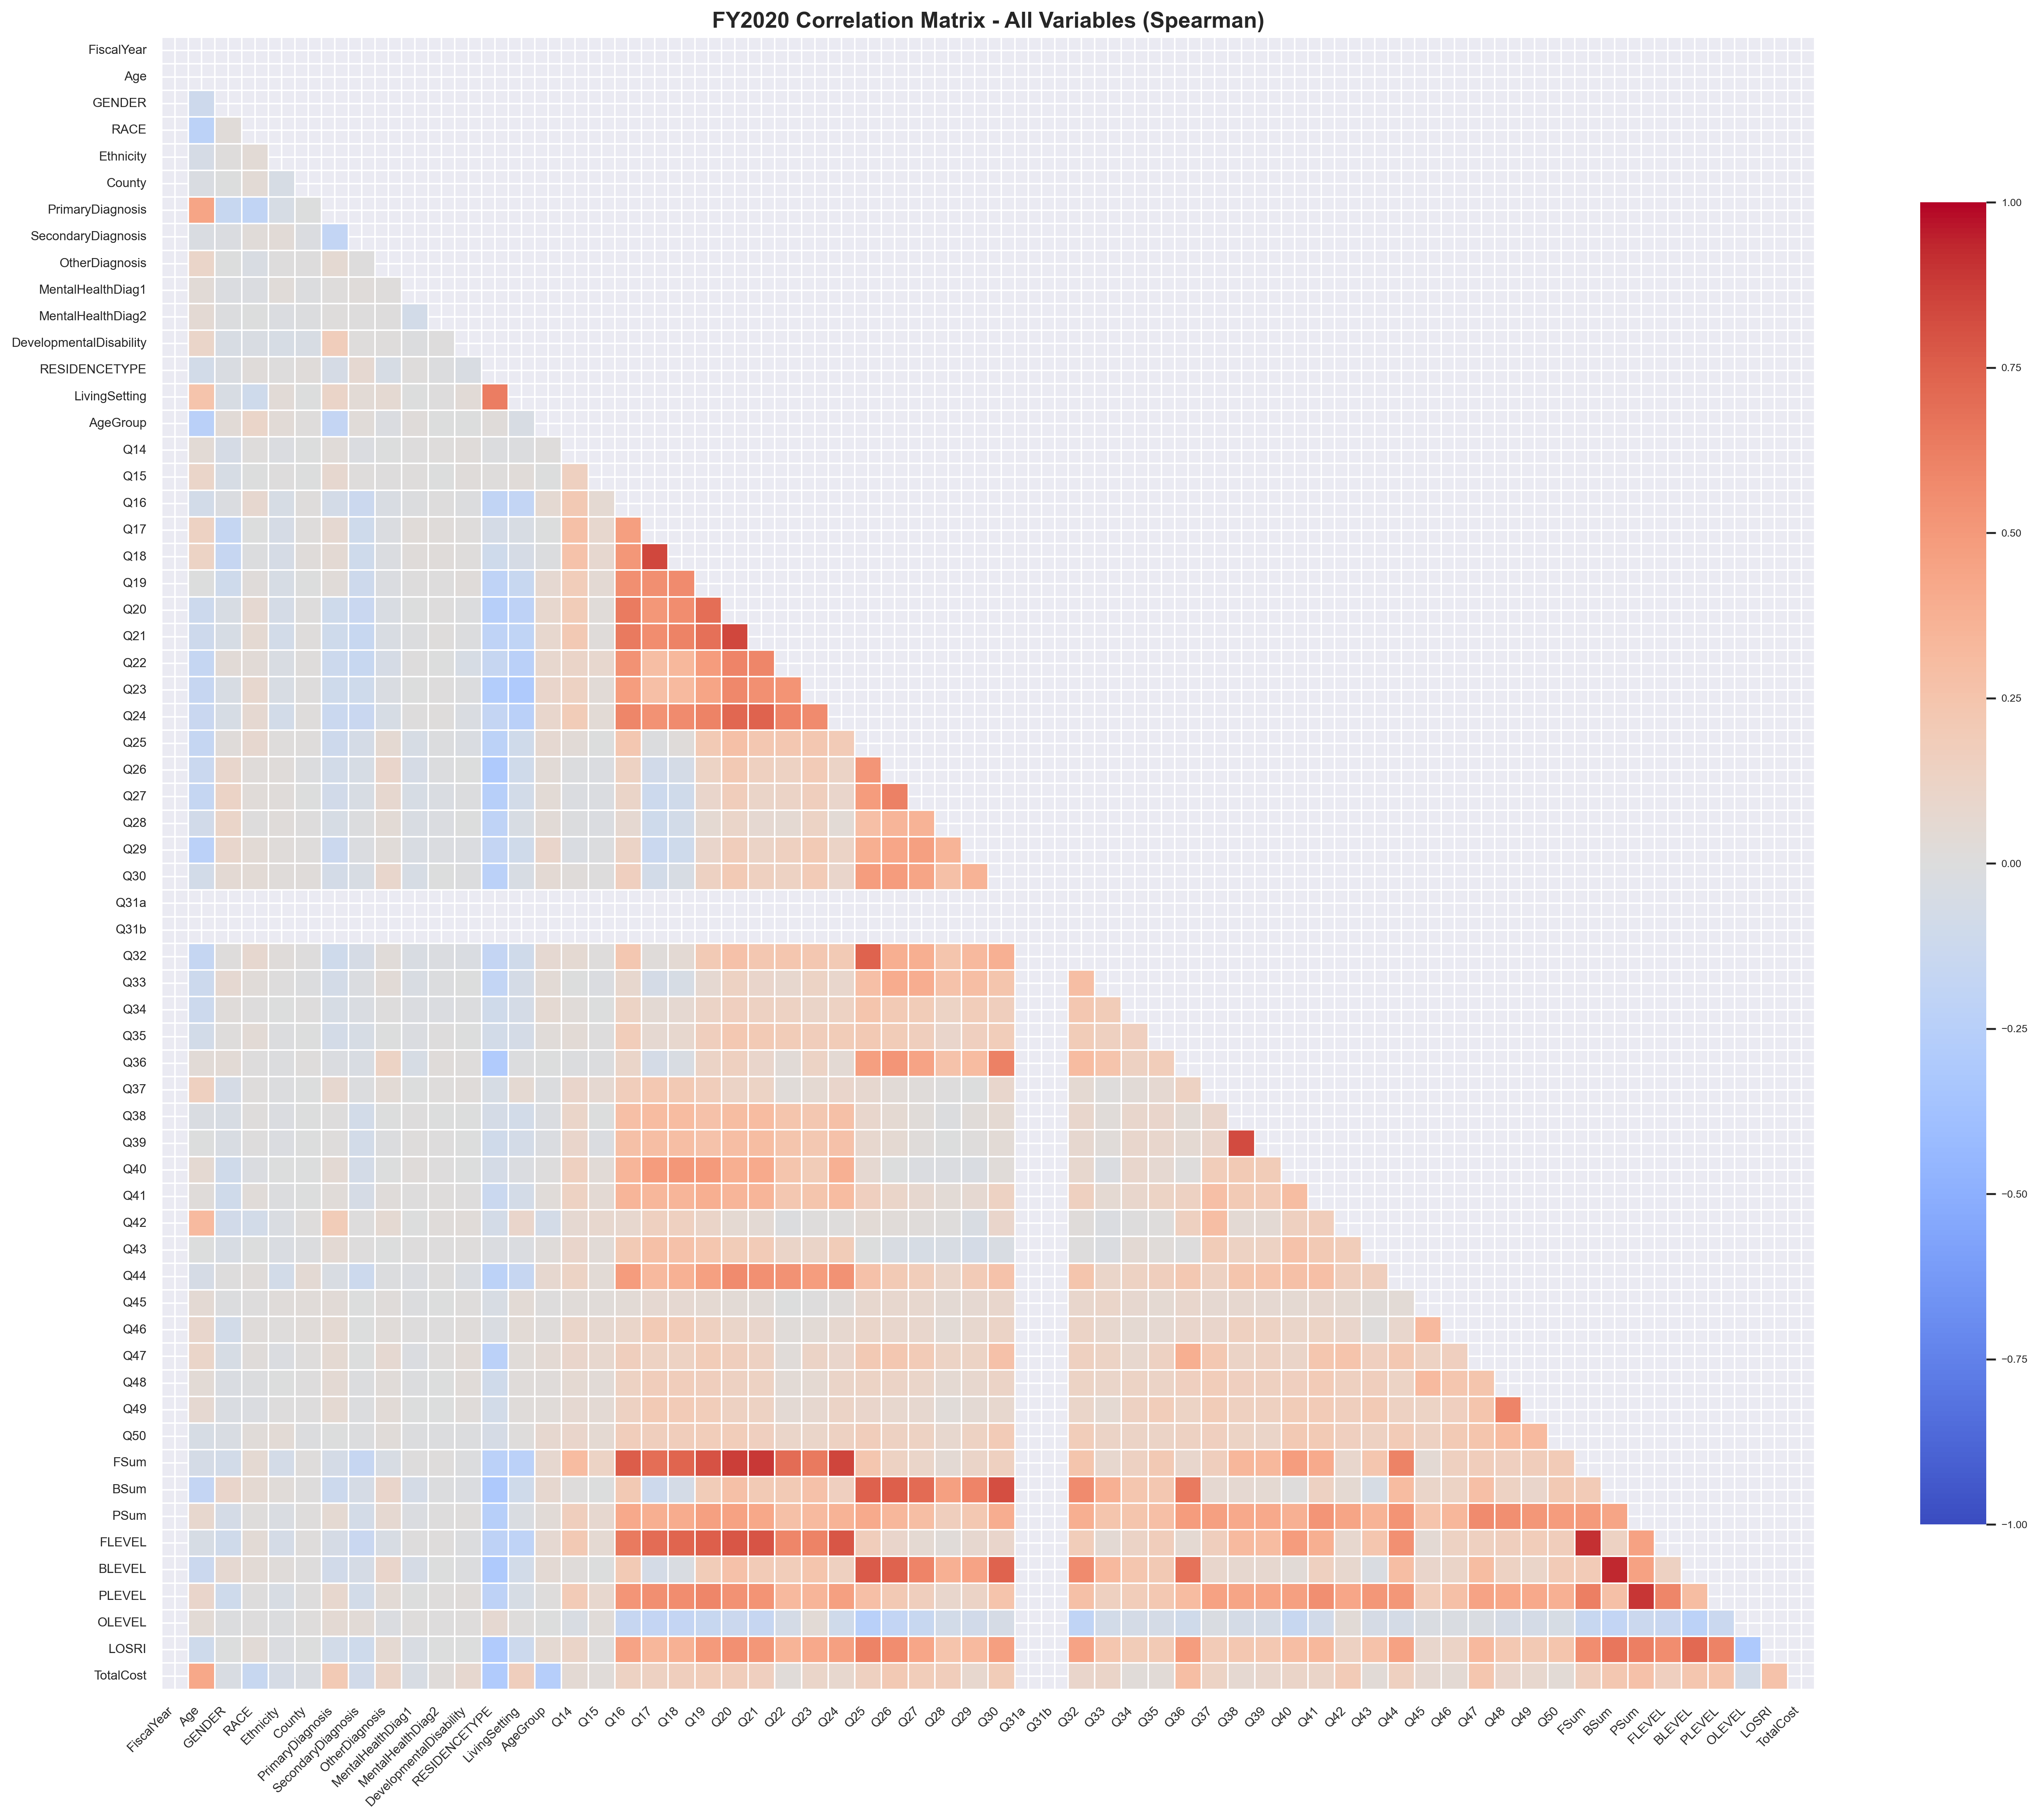
\includegraphics[width=\textwidth]{figures/fy2020_correlation_matrix_-_all_variables_(spearman).png}
    \caption{Spearman correlation matrix for all variables in FY2020, revealing complex interdependencies among QSI components and summary scores.}
    \label{fig:fy2020-corr-all}
\end{figure}

\newpage

\begin{figure}[htbp]
    \centering
    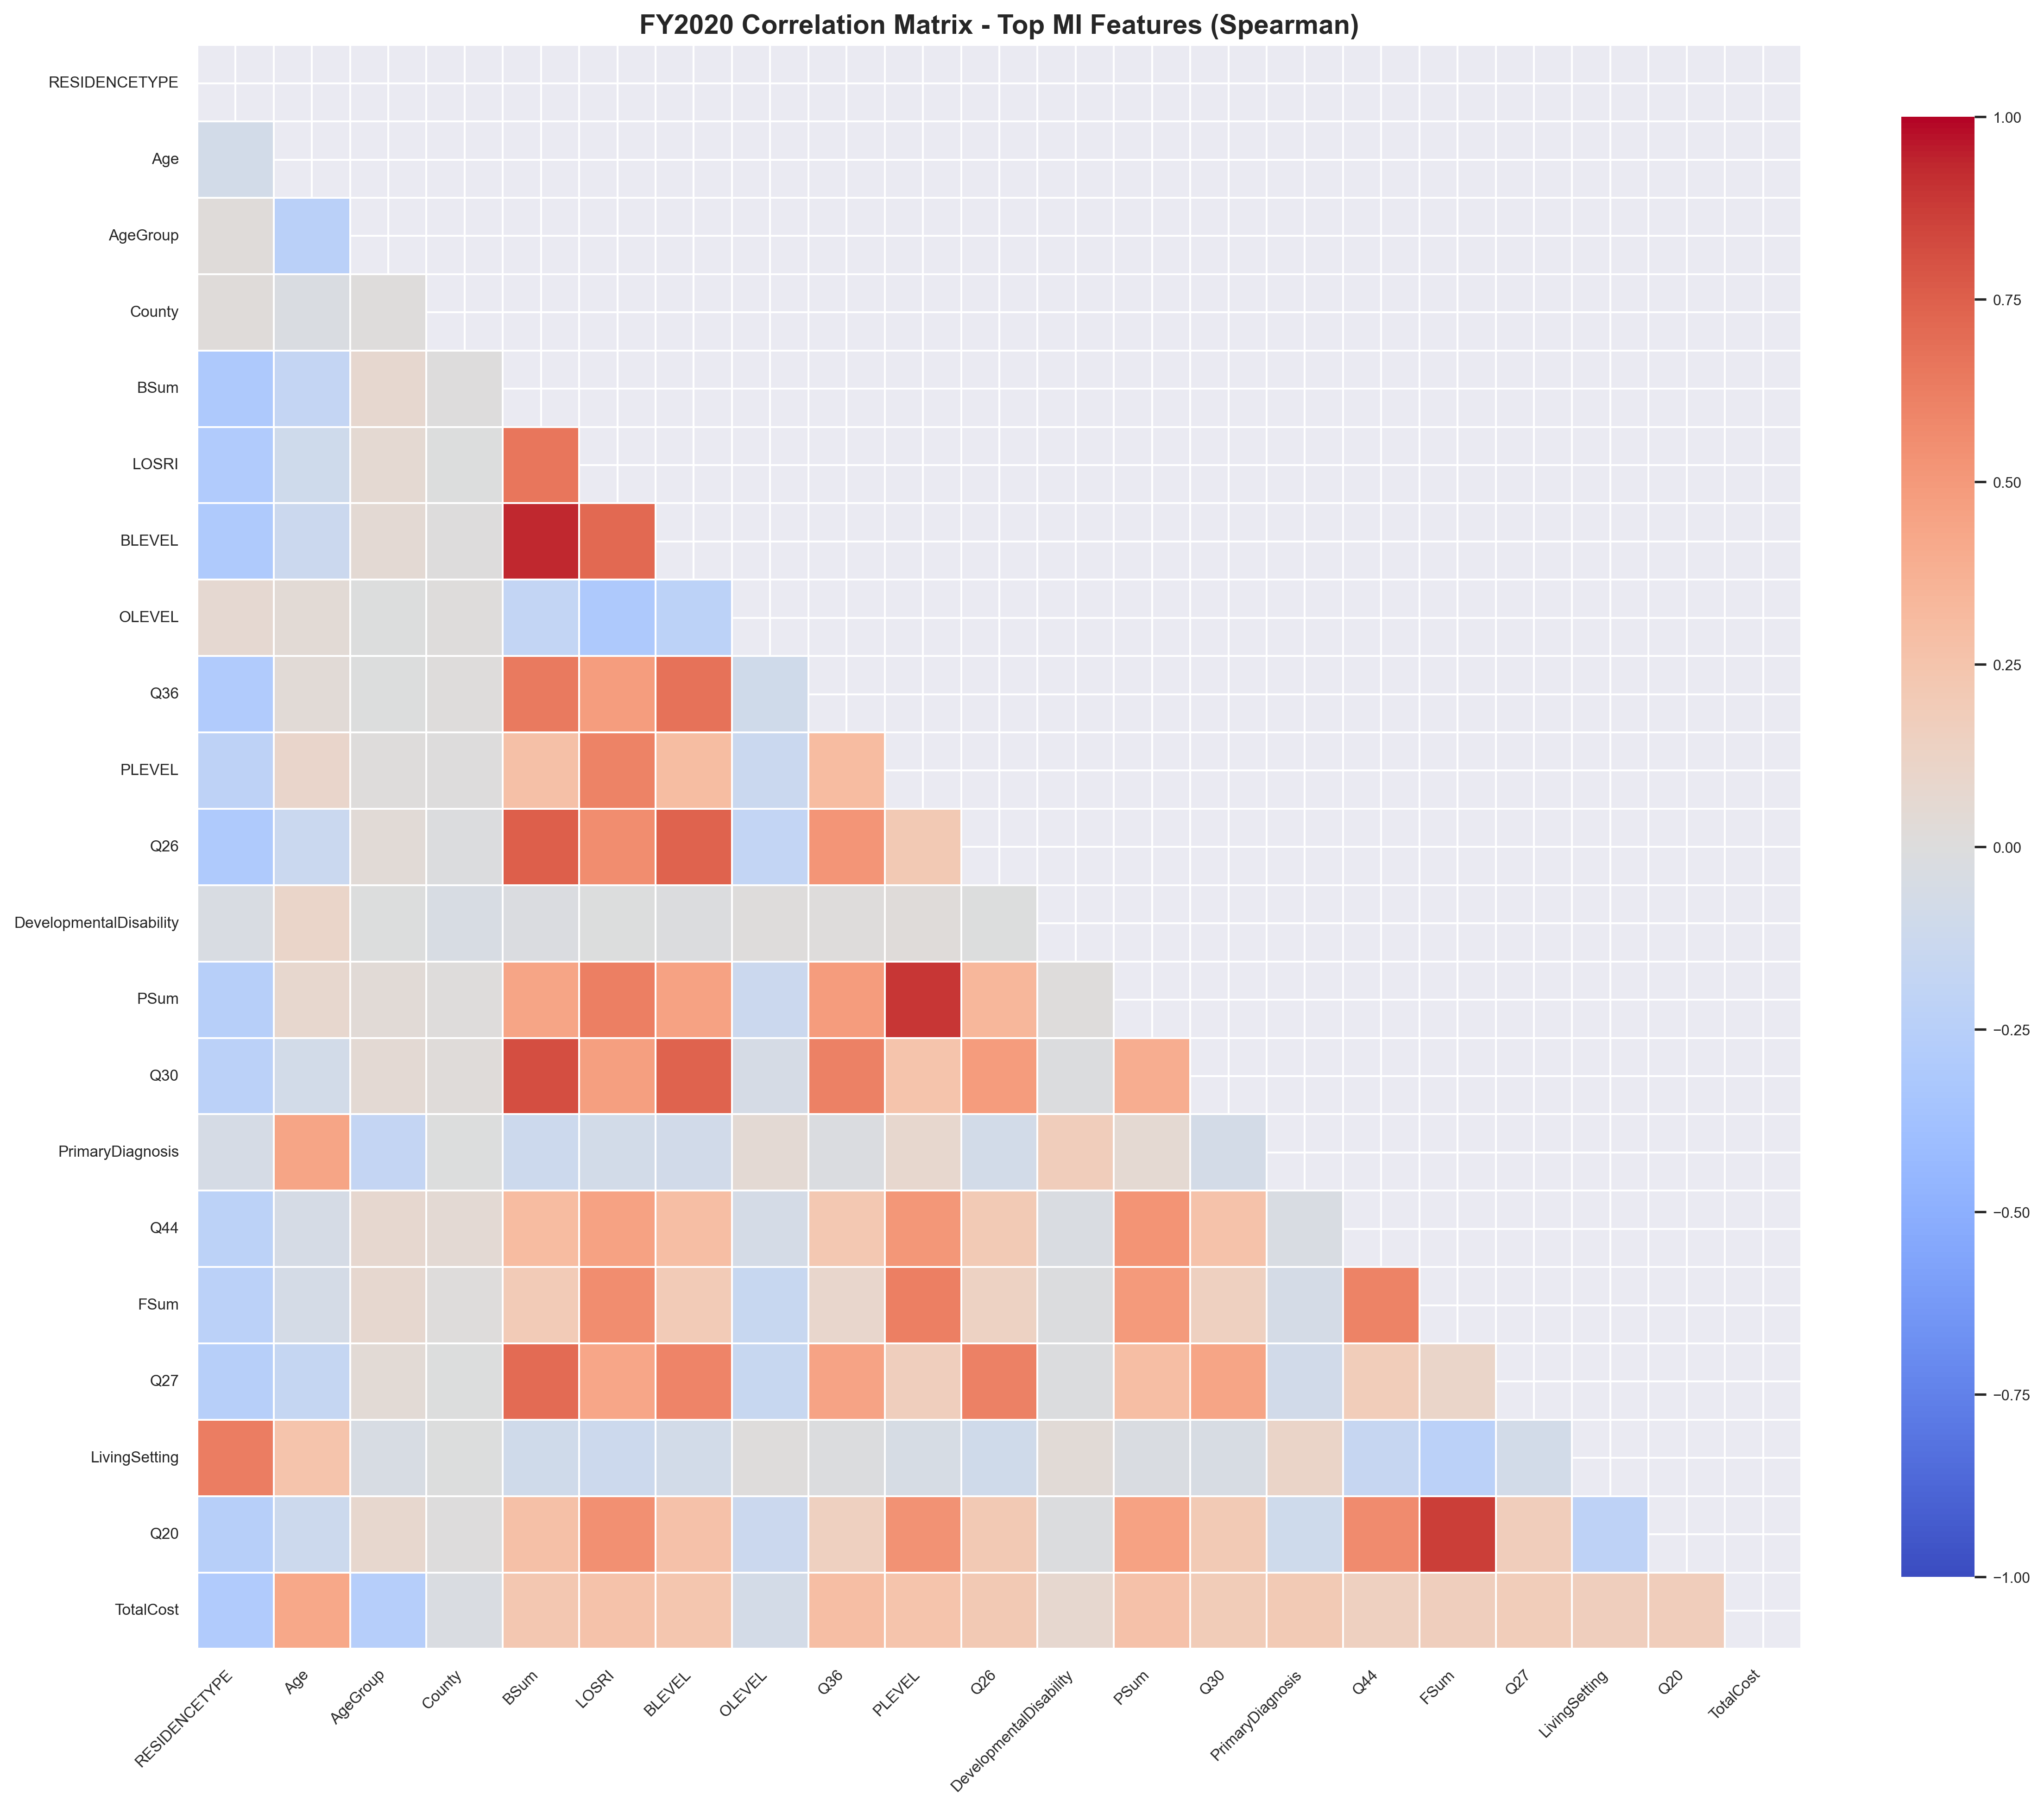
\includegraphics[width=0.9\textwidth]{figures/fy2020_correlation_matrix_-_top_mi_features_(spearman).png}
    \caption{Correlation structure among top 20 features ranked by mutual information for FY2020.}
    \label{fig:fy2020-corr-top}
\end{figure}

\newpage

\begin{figure}[htbp]
    \centering
    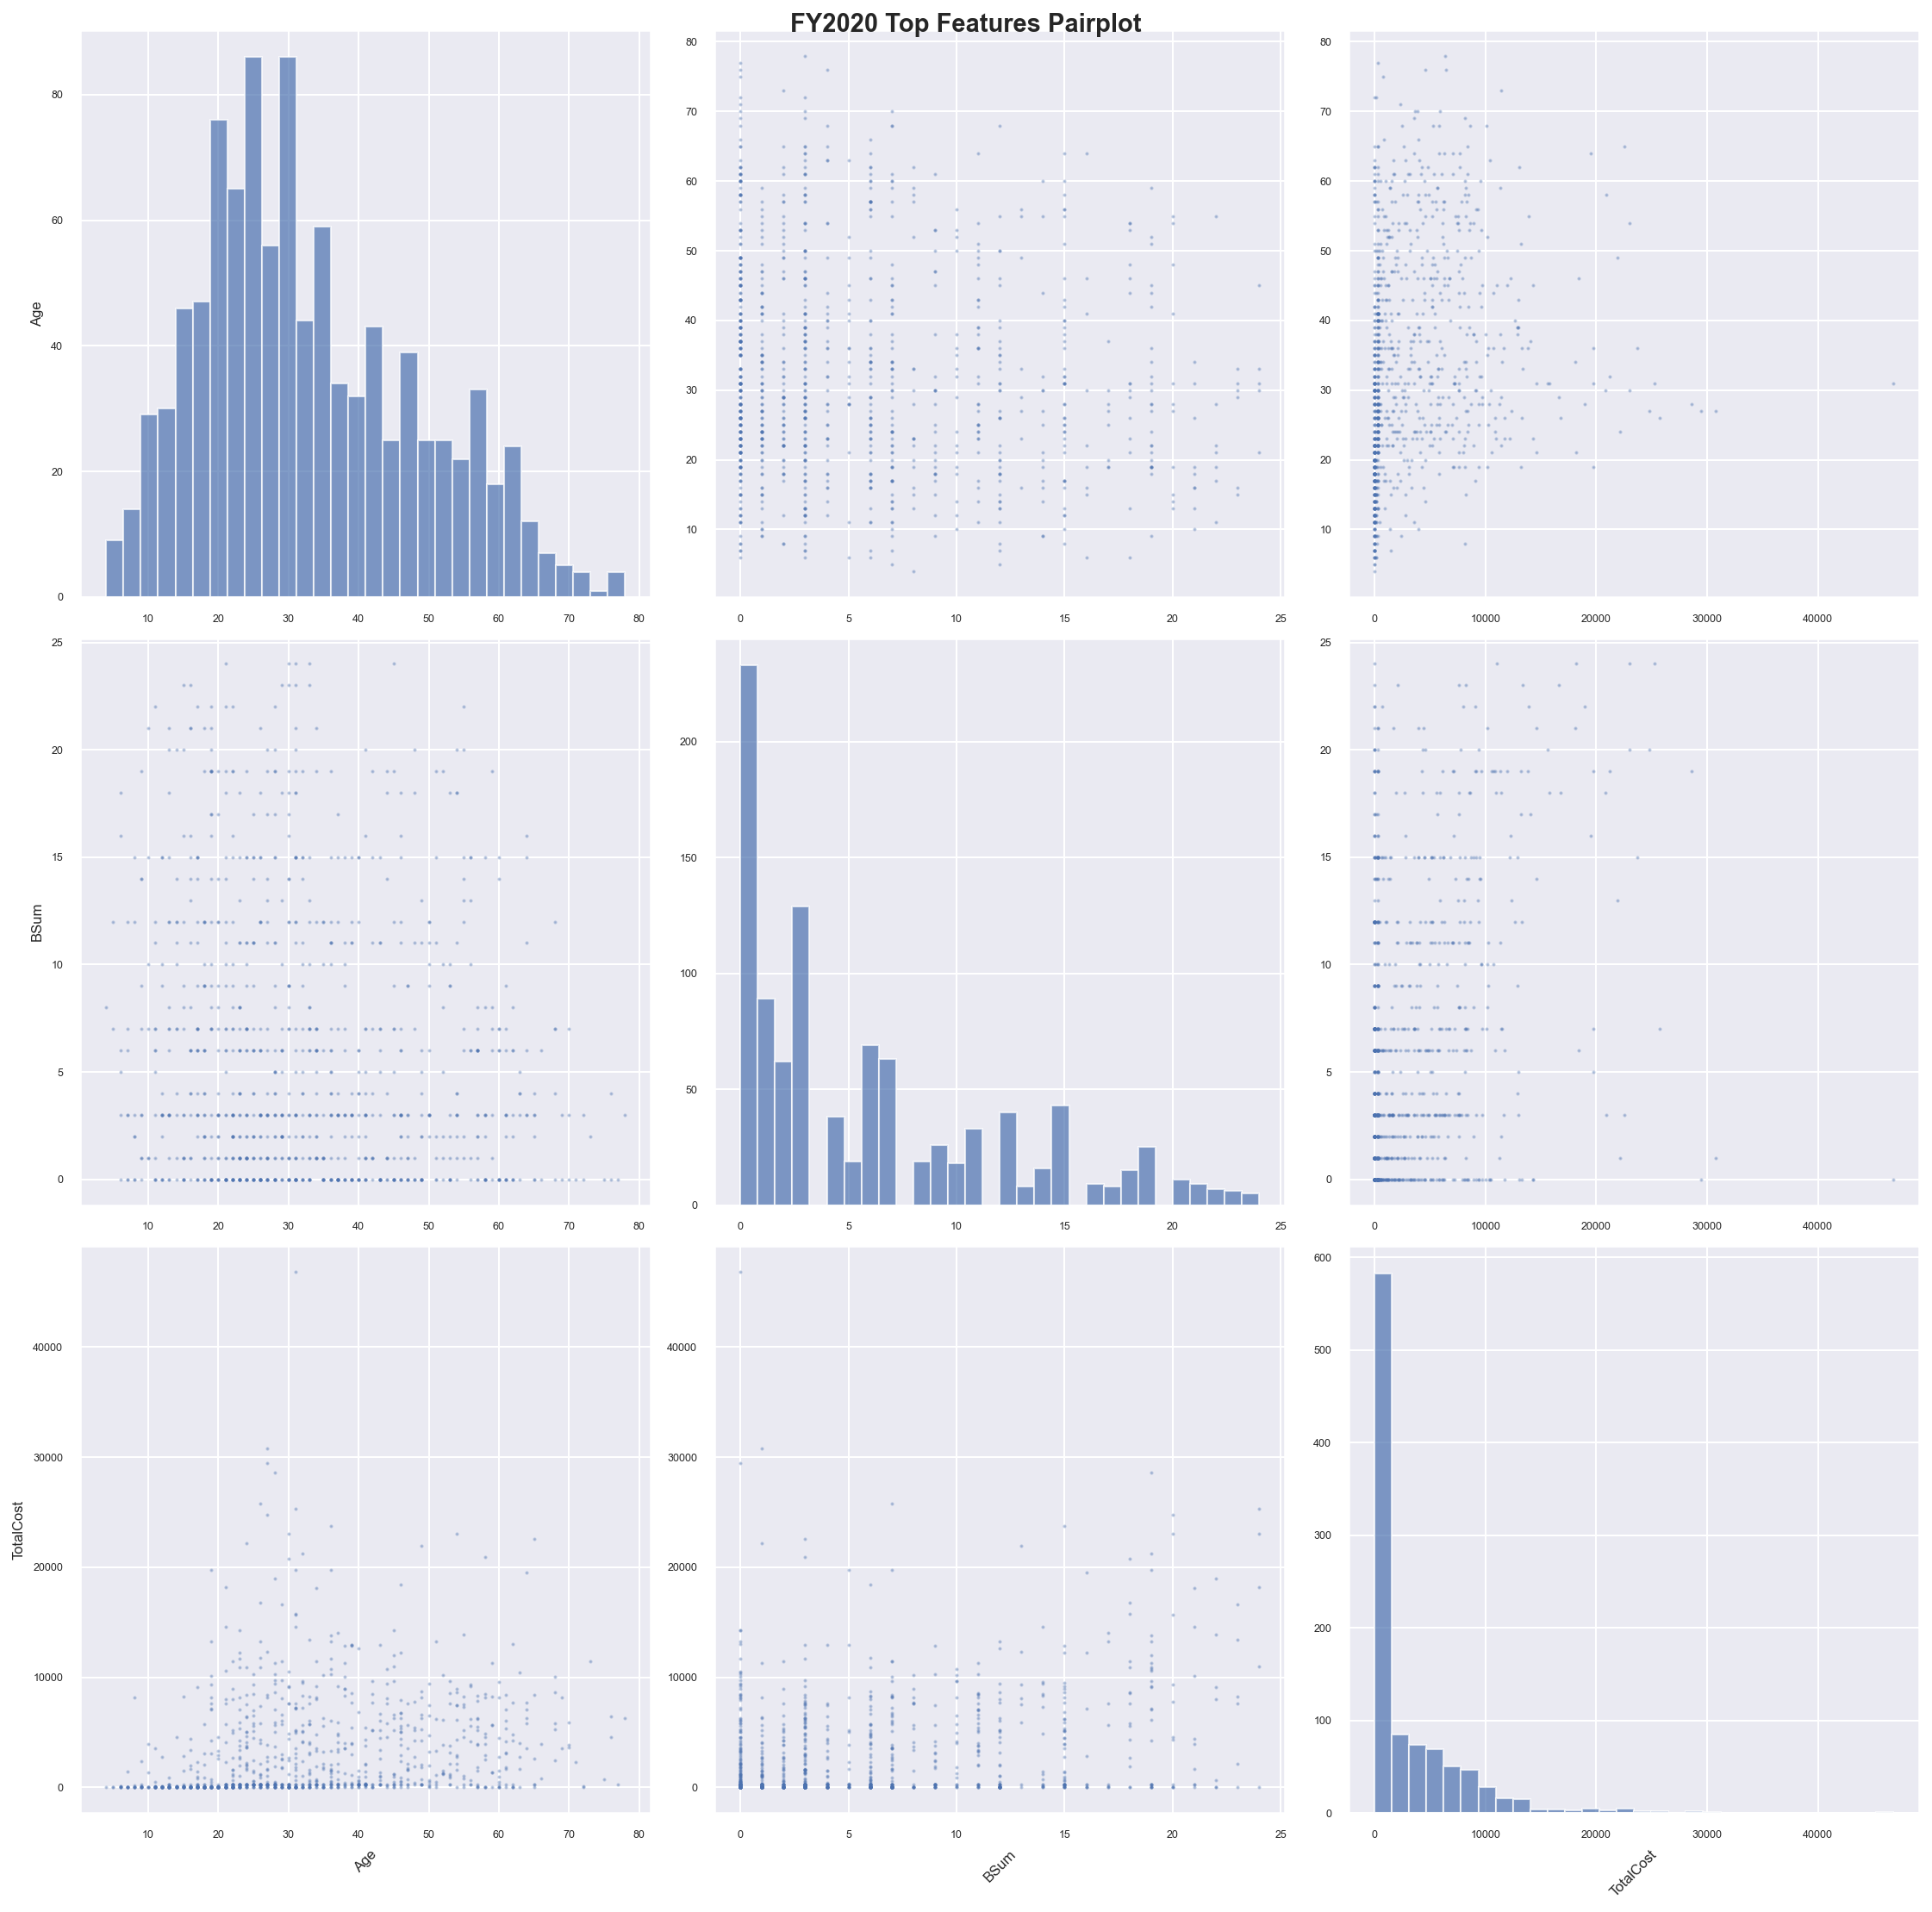
\includegraphics[width=\textwidth]{figures/fy2020_pairplot_top_features.png}
    \caption{Pairwise relationships among top predictive features for FY2020, showing non-linear patterns and heteroscedasticity.}
    \label{fig:fy2020-pairplot}
\end{figure}

\newpage

\subsection{Fiscal Year 2021}
\label{subsec:fy2021}

The FY2021 analysis (n=20,541) demonstrated consistency in top predictors, with \texttt{RESIDENCETYPE} maintaining the highest MI score (0.2597). Notable changes included increased importance of \texttt{LOSRI} (MI=0.1132) and \texttt{OLEVEL} (MI=0.1131), suggesting evolving relationships between support levels and costs following the COVID-19 pandemic's impact on service delivery.

\begin{figure}[htbp]
    \centering
    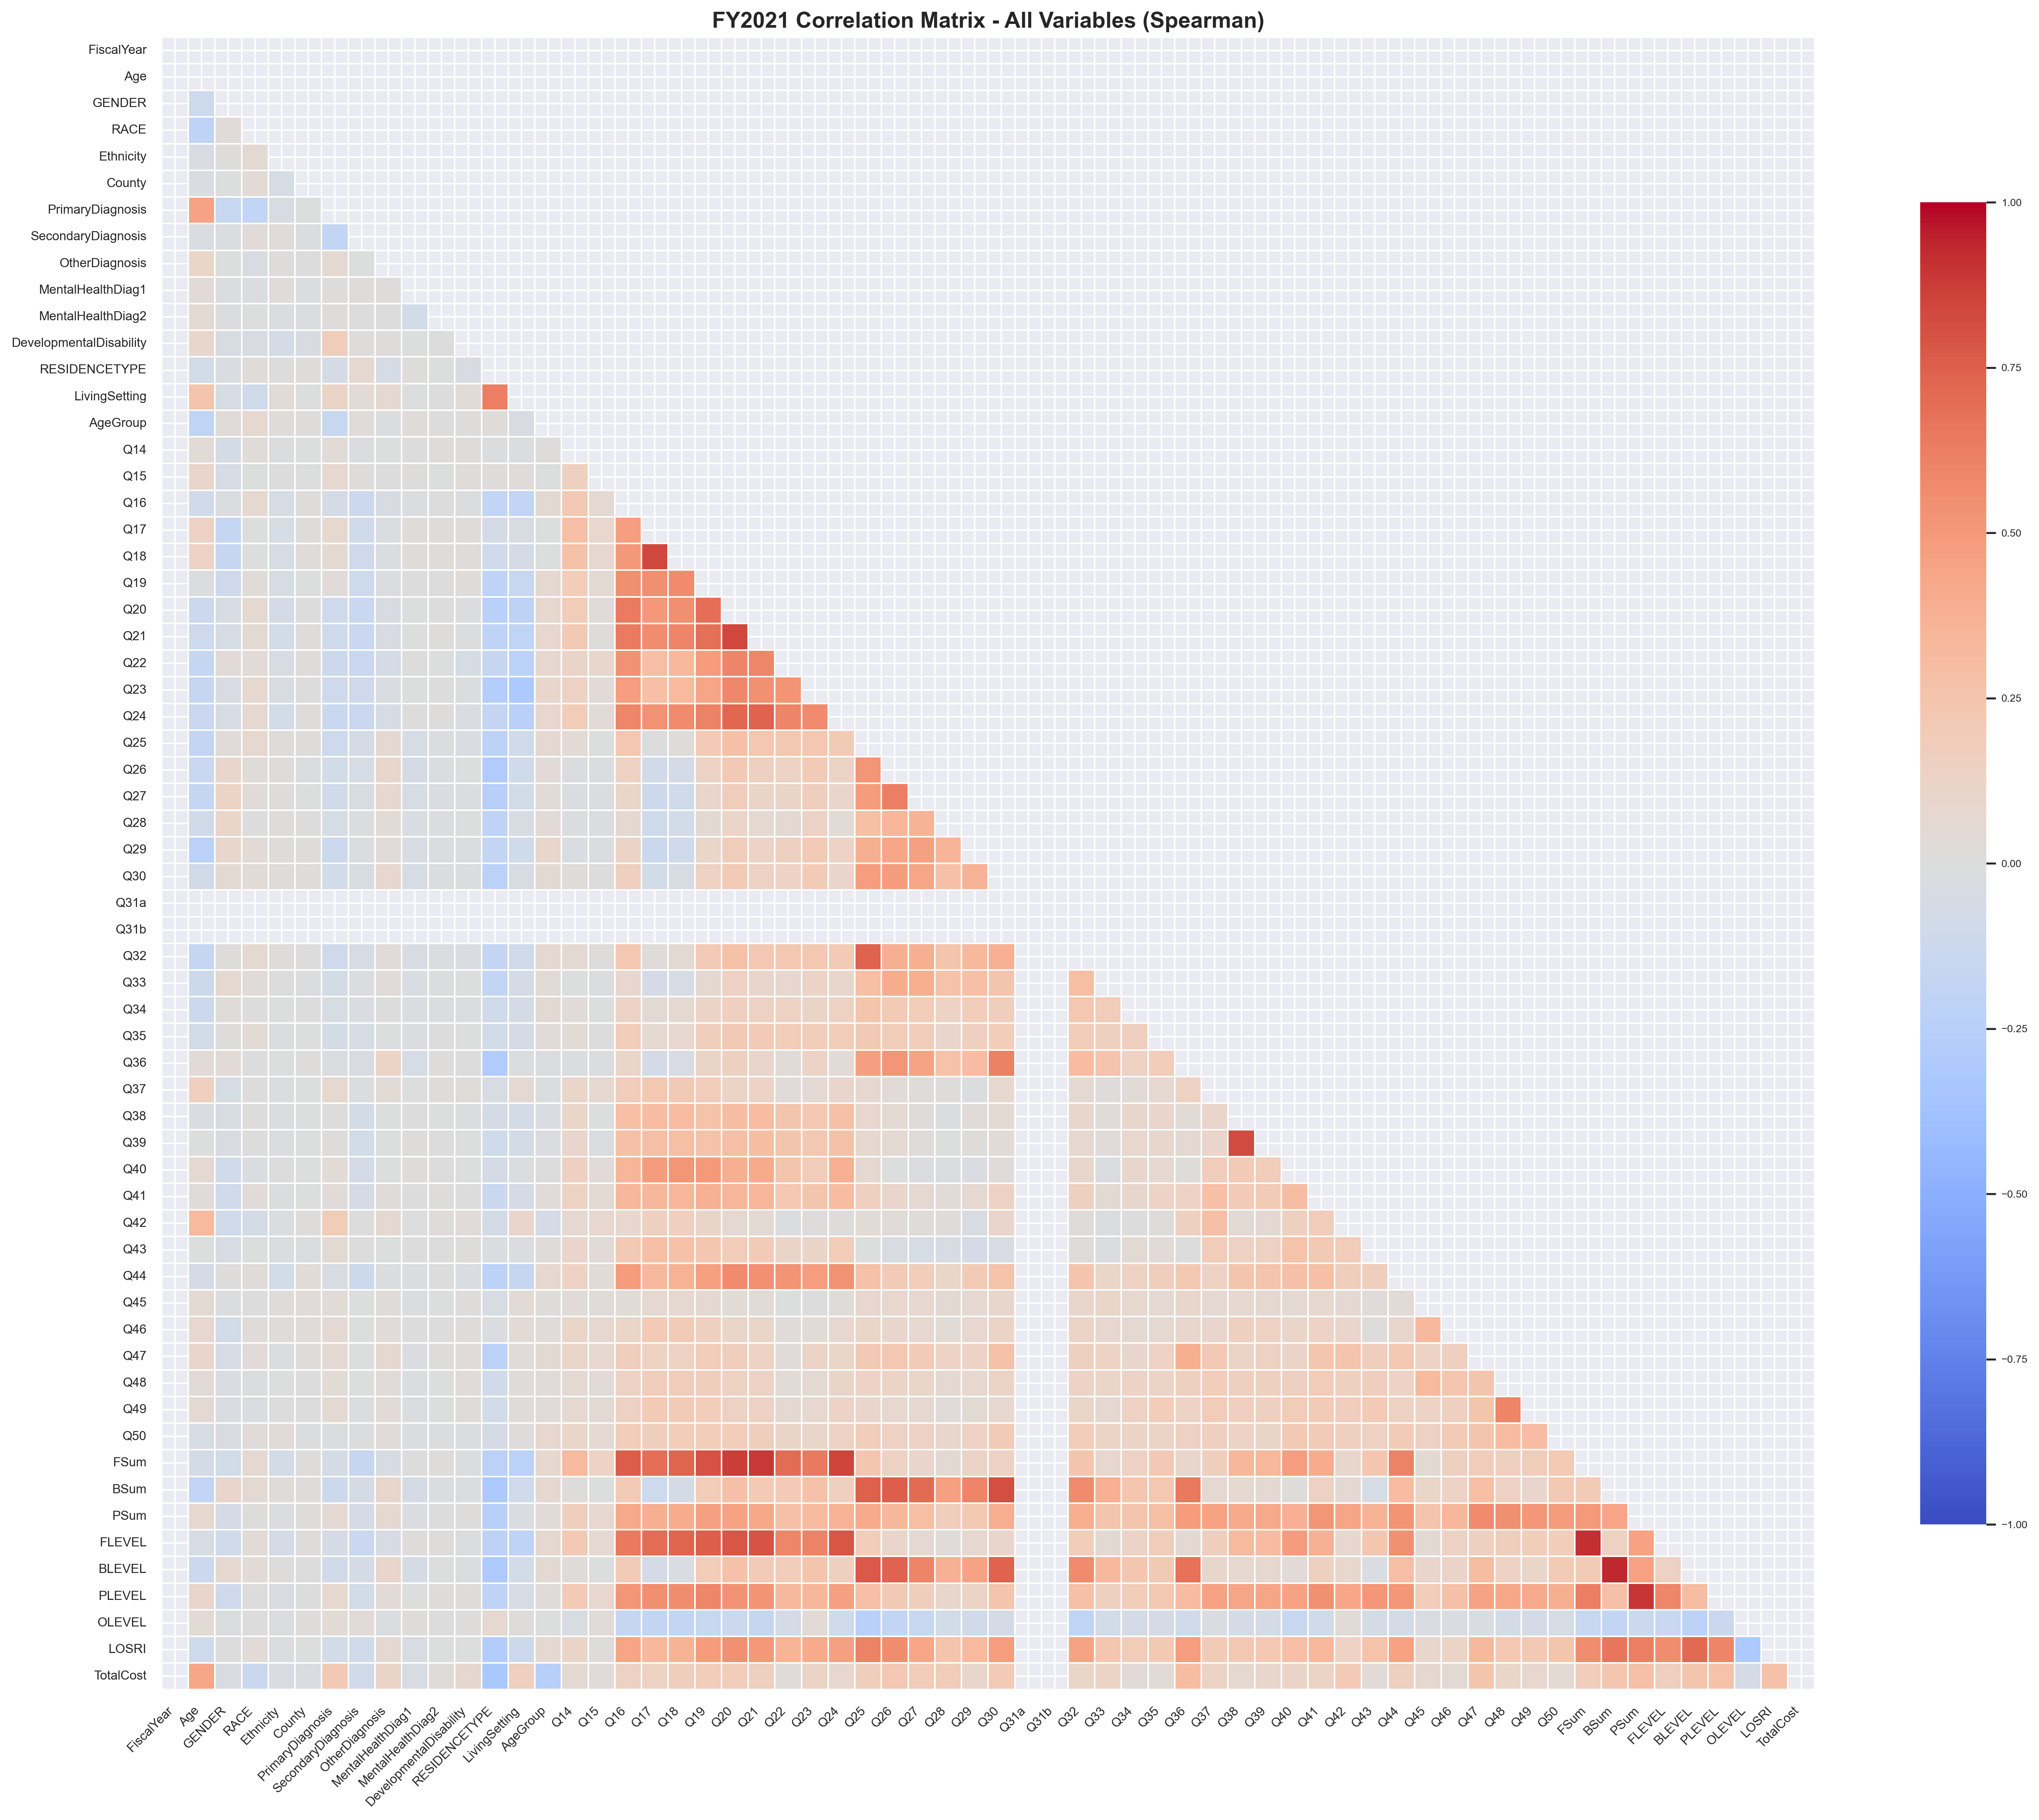
\includegraphics[width=\textwidth]{figures/fy2021_correlation_matrix_-_all_variables_(spearman).png}
    \caption{Complete correlation structure for FY2021 variables.}
    \label{fig:fy2021-corr-all}
\end{figure}

\newpage

\subsection{Fiscal Year 2022}
\label{subsec:fy2022}

Analysis of FY2022 data (n=21,063) revealed further strengthening of \texttt{RESIDENCETYPE}'s predictive power (MI=0.2719). The behavioral and functional assessment components maintained strong relationships with costs, while geographic variation (\texttt{County}) remained a significant factor (MI=0.0797).

\begin{figure}[htbp]
    \centering
    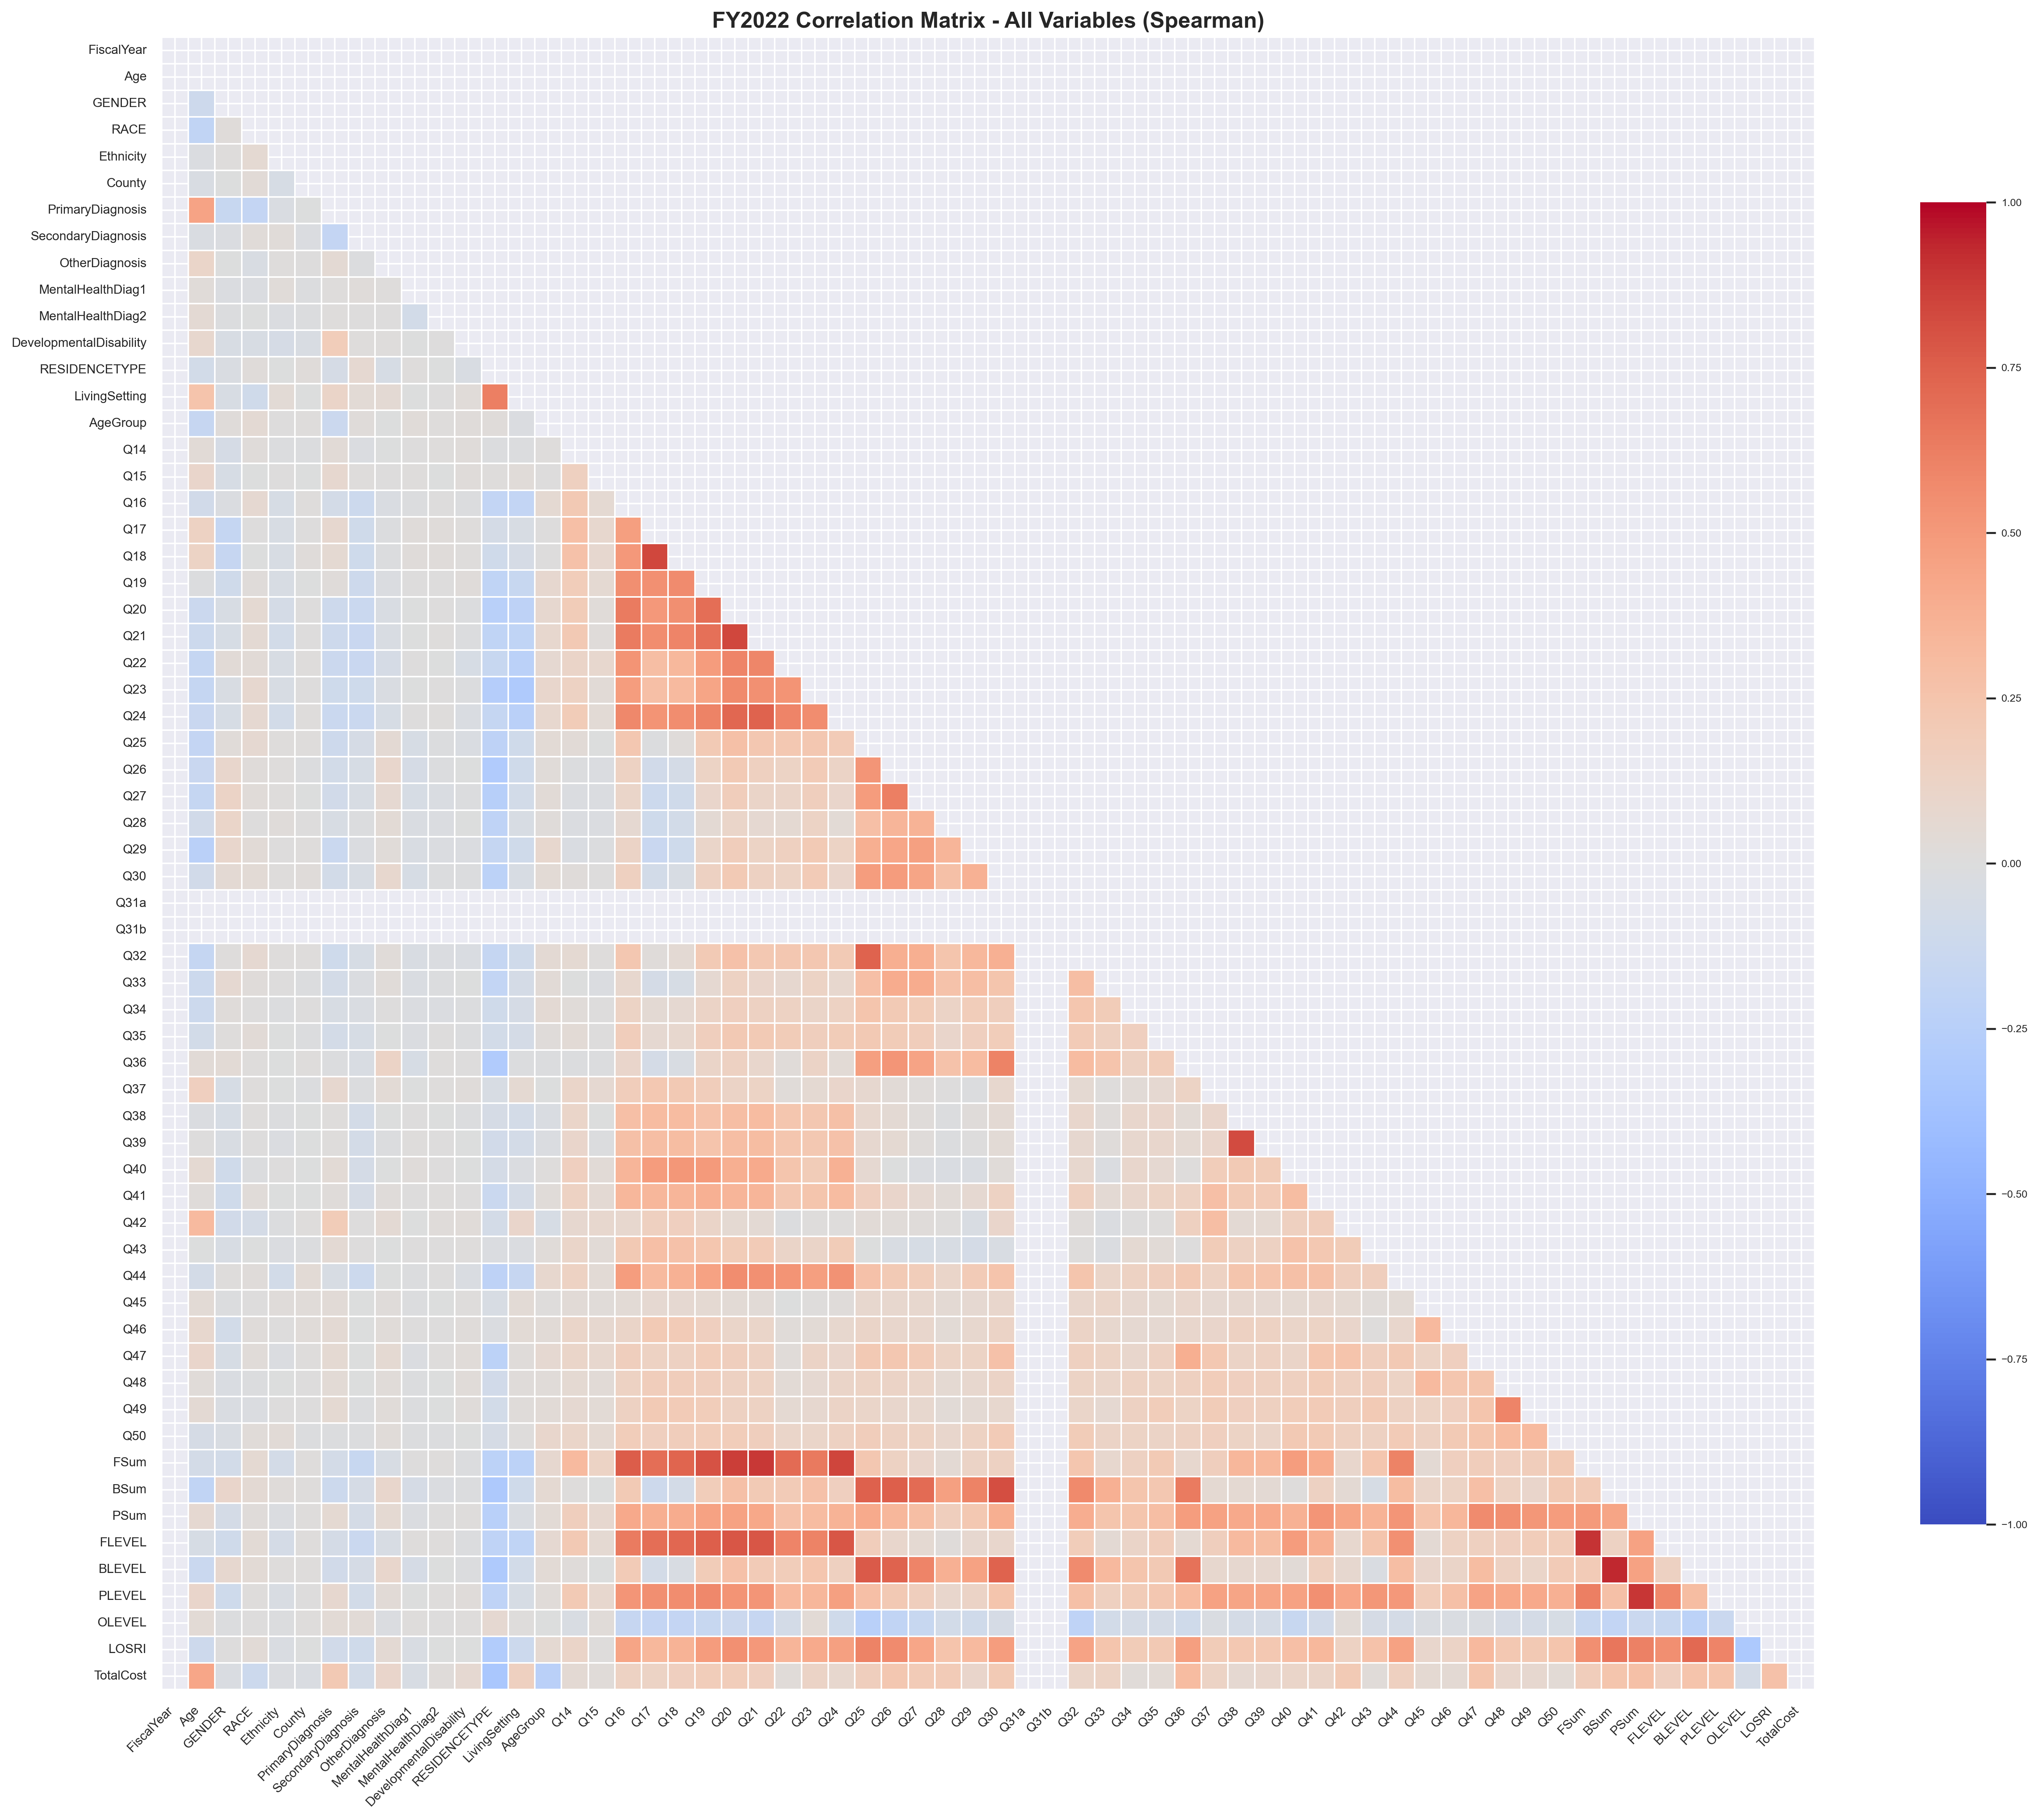
\includegraphics[width=\textwidth]{figures/fy2022_correlation_matrix_-_all_variables_(spearman).png}
    \caption{Correlation matrix for FY2022 showing stability in feature relationships.}
    \label{fig:fy2022-corr-all}
\end{figure}

\newpage

\subsection{Fiscal Year 2023}
\label{subsec:fy2023}

The FY2023 cohort (n=22,293) exhibited similar patterns with \texttt{RESIDENCETYPE} (MI=0.2520), though \texttt{LOSRI} emerged as the second-strongest predictor (MI=0.1304), surpassing behavioral measures. This shift suggested increasing importance of comprehensive support level assessments.

\begin{figure}[htbp]
    \centering
    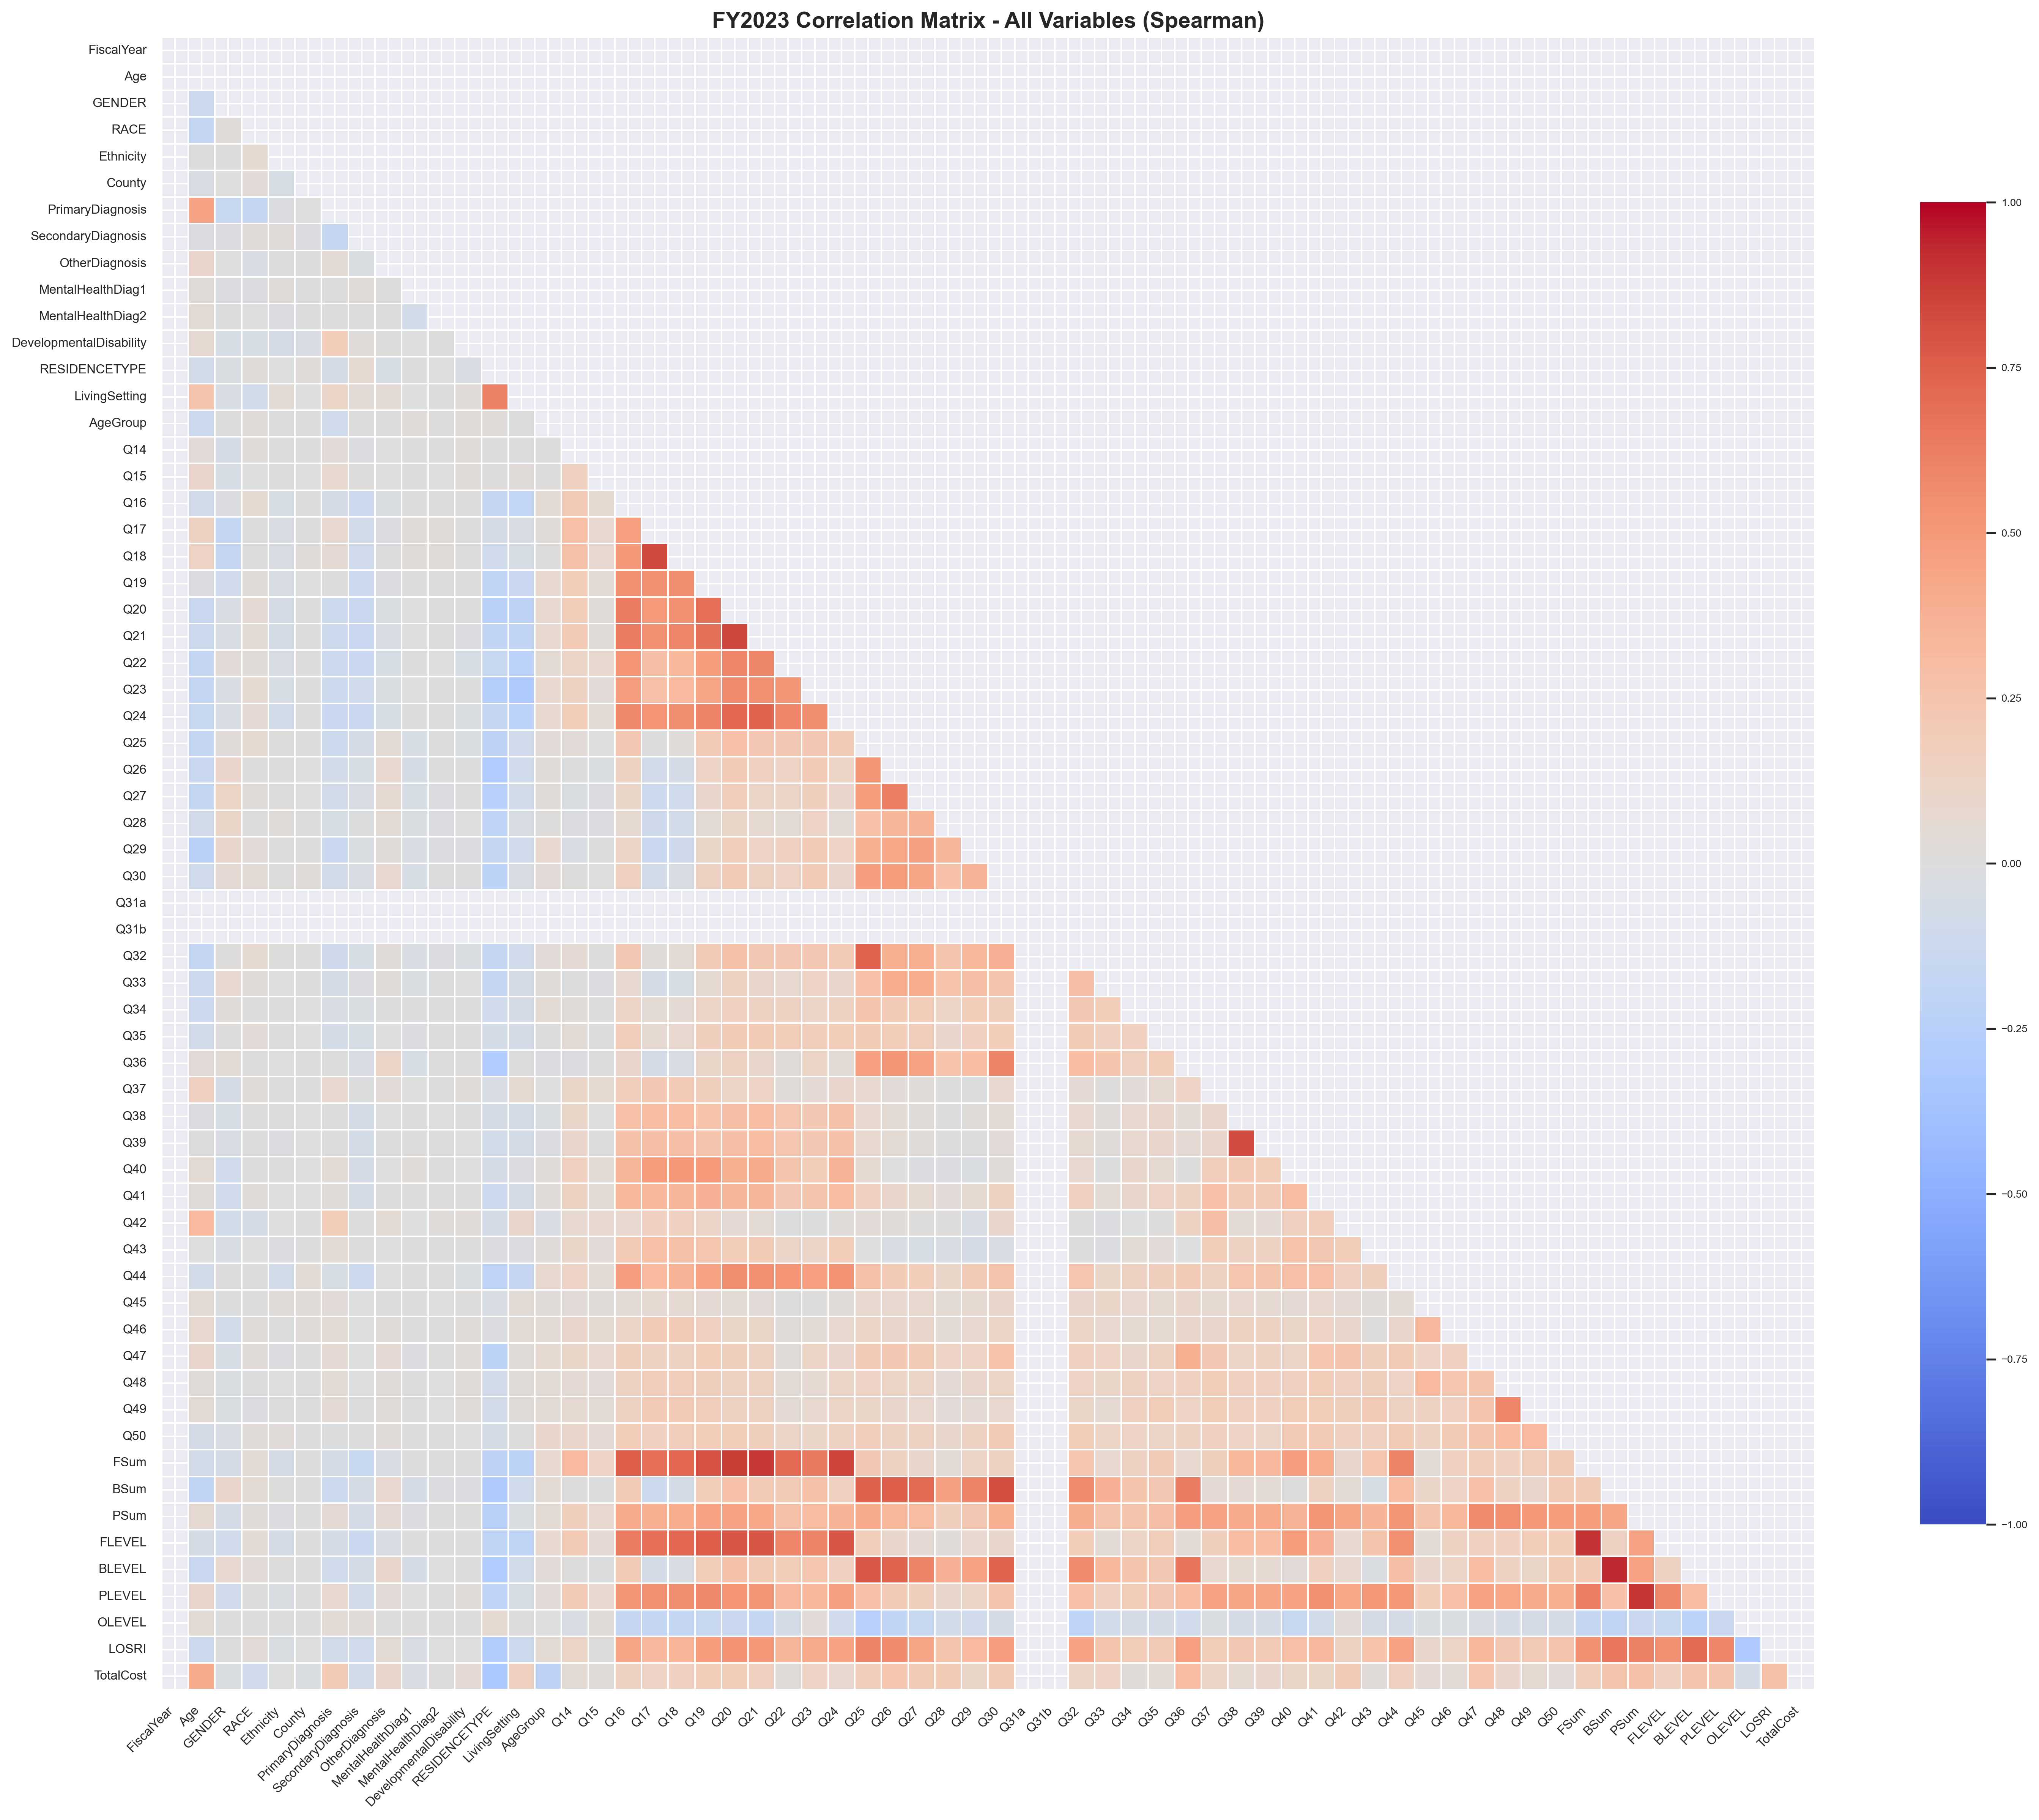
\includegraphics[width=\textwidth]{figures/fy2023_correlation_matrix_-_all_variables_(spearman).png}
    \caption{FY2023 correlation structure demonstrating evolving feature importance.}
    \label{fig:fy2023-corr-all}
\end{figure}

\newpage

\subsection{Fiscal Year 2024}
\label{subsec:fy2024}

FY2024 data (n=23,251) maintained consistent patterns with \texttt{RESIDENCETYPE} (MI=0.2554) and support level indicators dominating predictions. The stability of mutual information scores across consecutive years validated the robustness of identified relationships.

\begin{figure}[htbp]
    \centering
    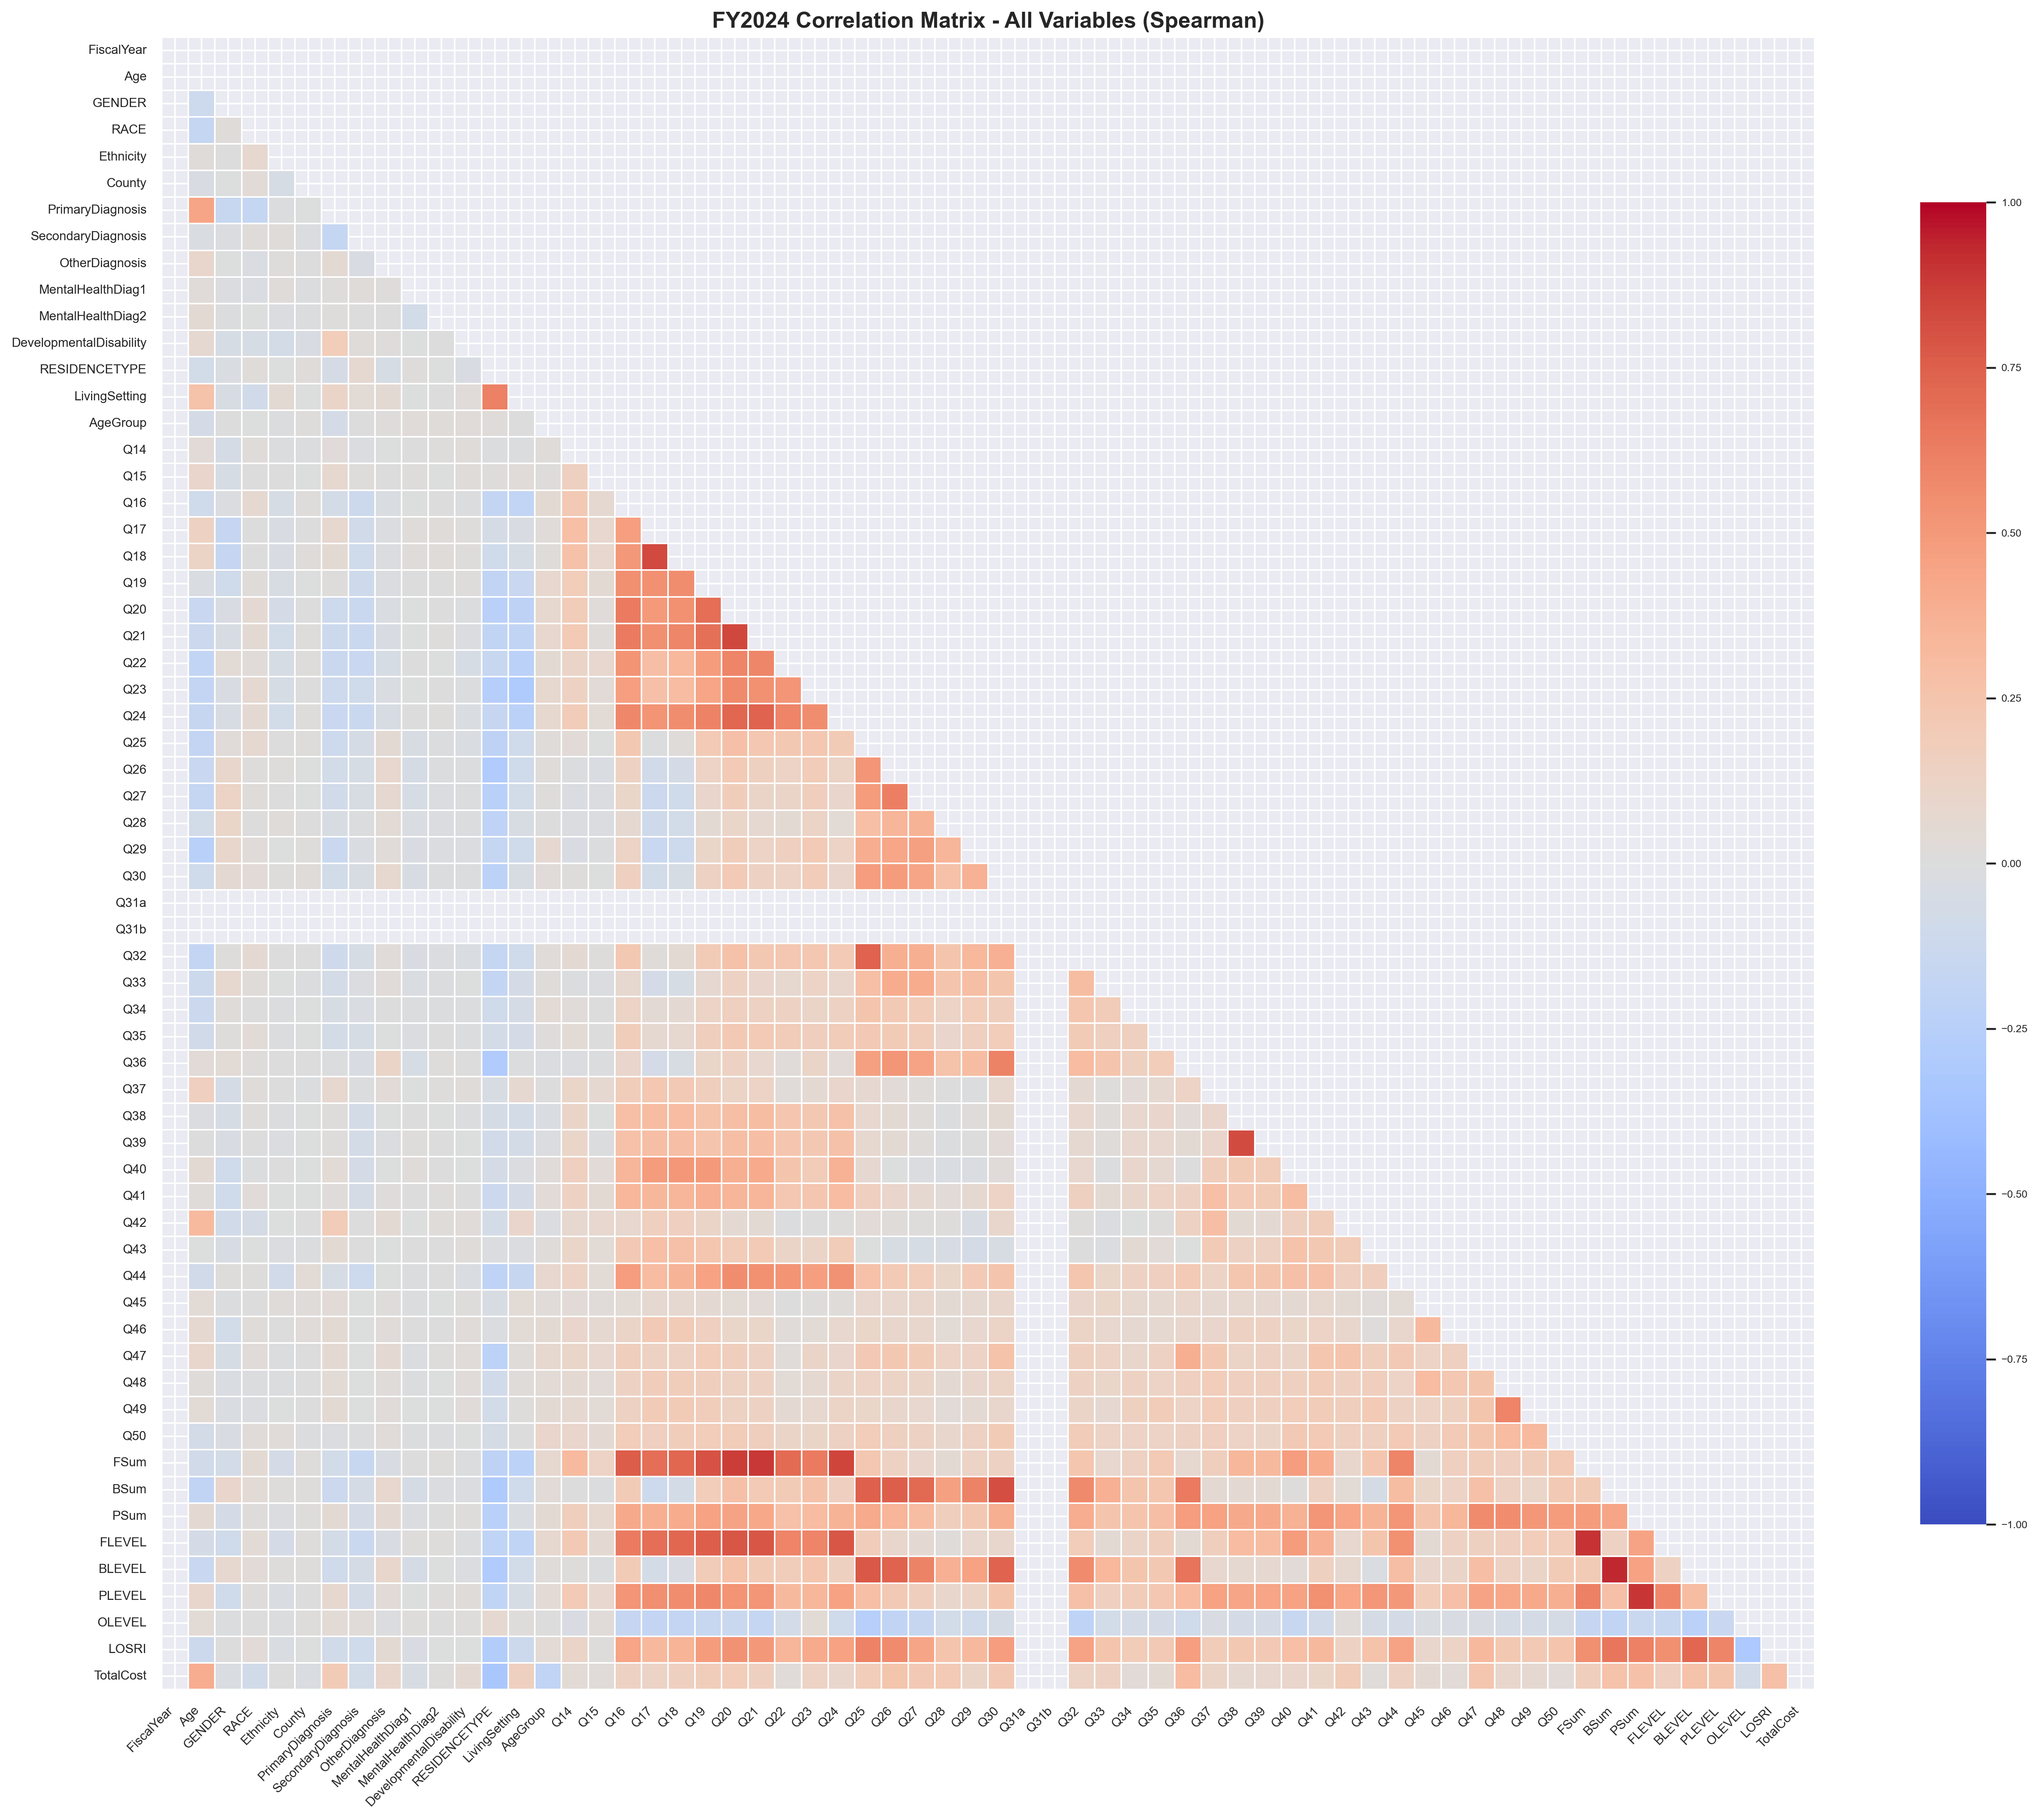
\includegraphics[width=\textwidth]{figures/fy2024_correlation_matrix_-_all_variables_(spearman).png}
    \caption{Correlation analysis for FY2024 confirming persistent feature relationships.}
    \label{fig:fy2024-corr-all}
\end{figure}

\newpage

\subsection{Fiscal Year 2025}
\label{subsec:fy2025}

The most recent complete fiscal year (FY2025, n=23,792) demonstrated remarkable consistency in feature importance rankings, with \texttt{RESIDENCETYPE} (MI=0.2590), \texttt{BSum} (MI=0.1367), and support level indicators maintaining their predictive dominance.

\begin{figure}[htbp]
    \centering
    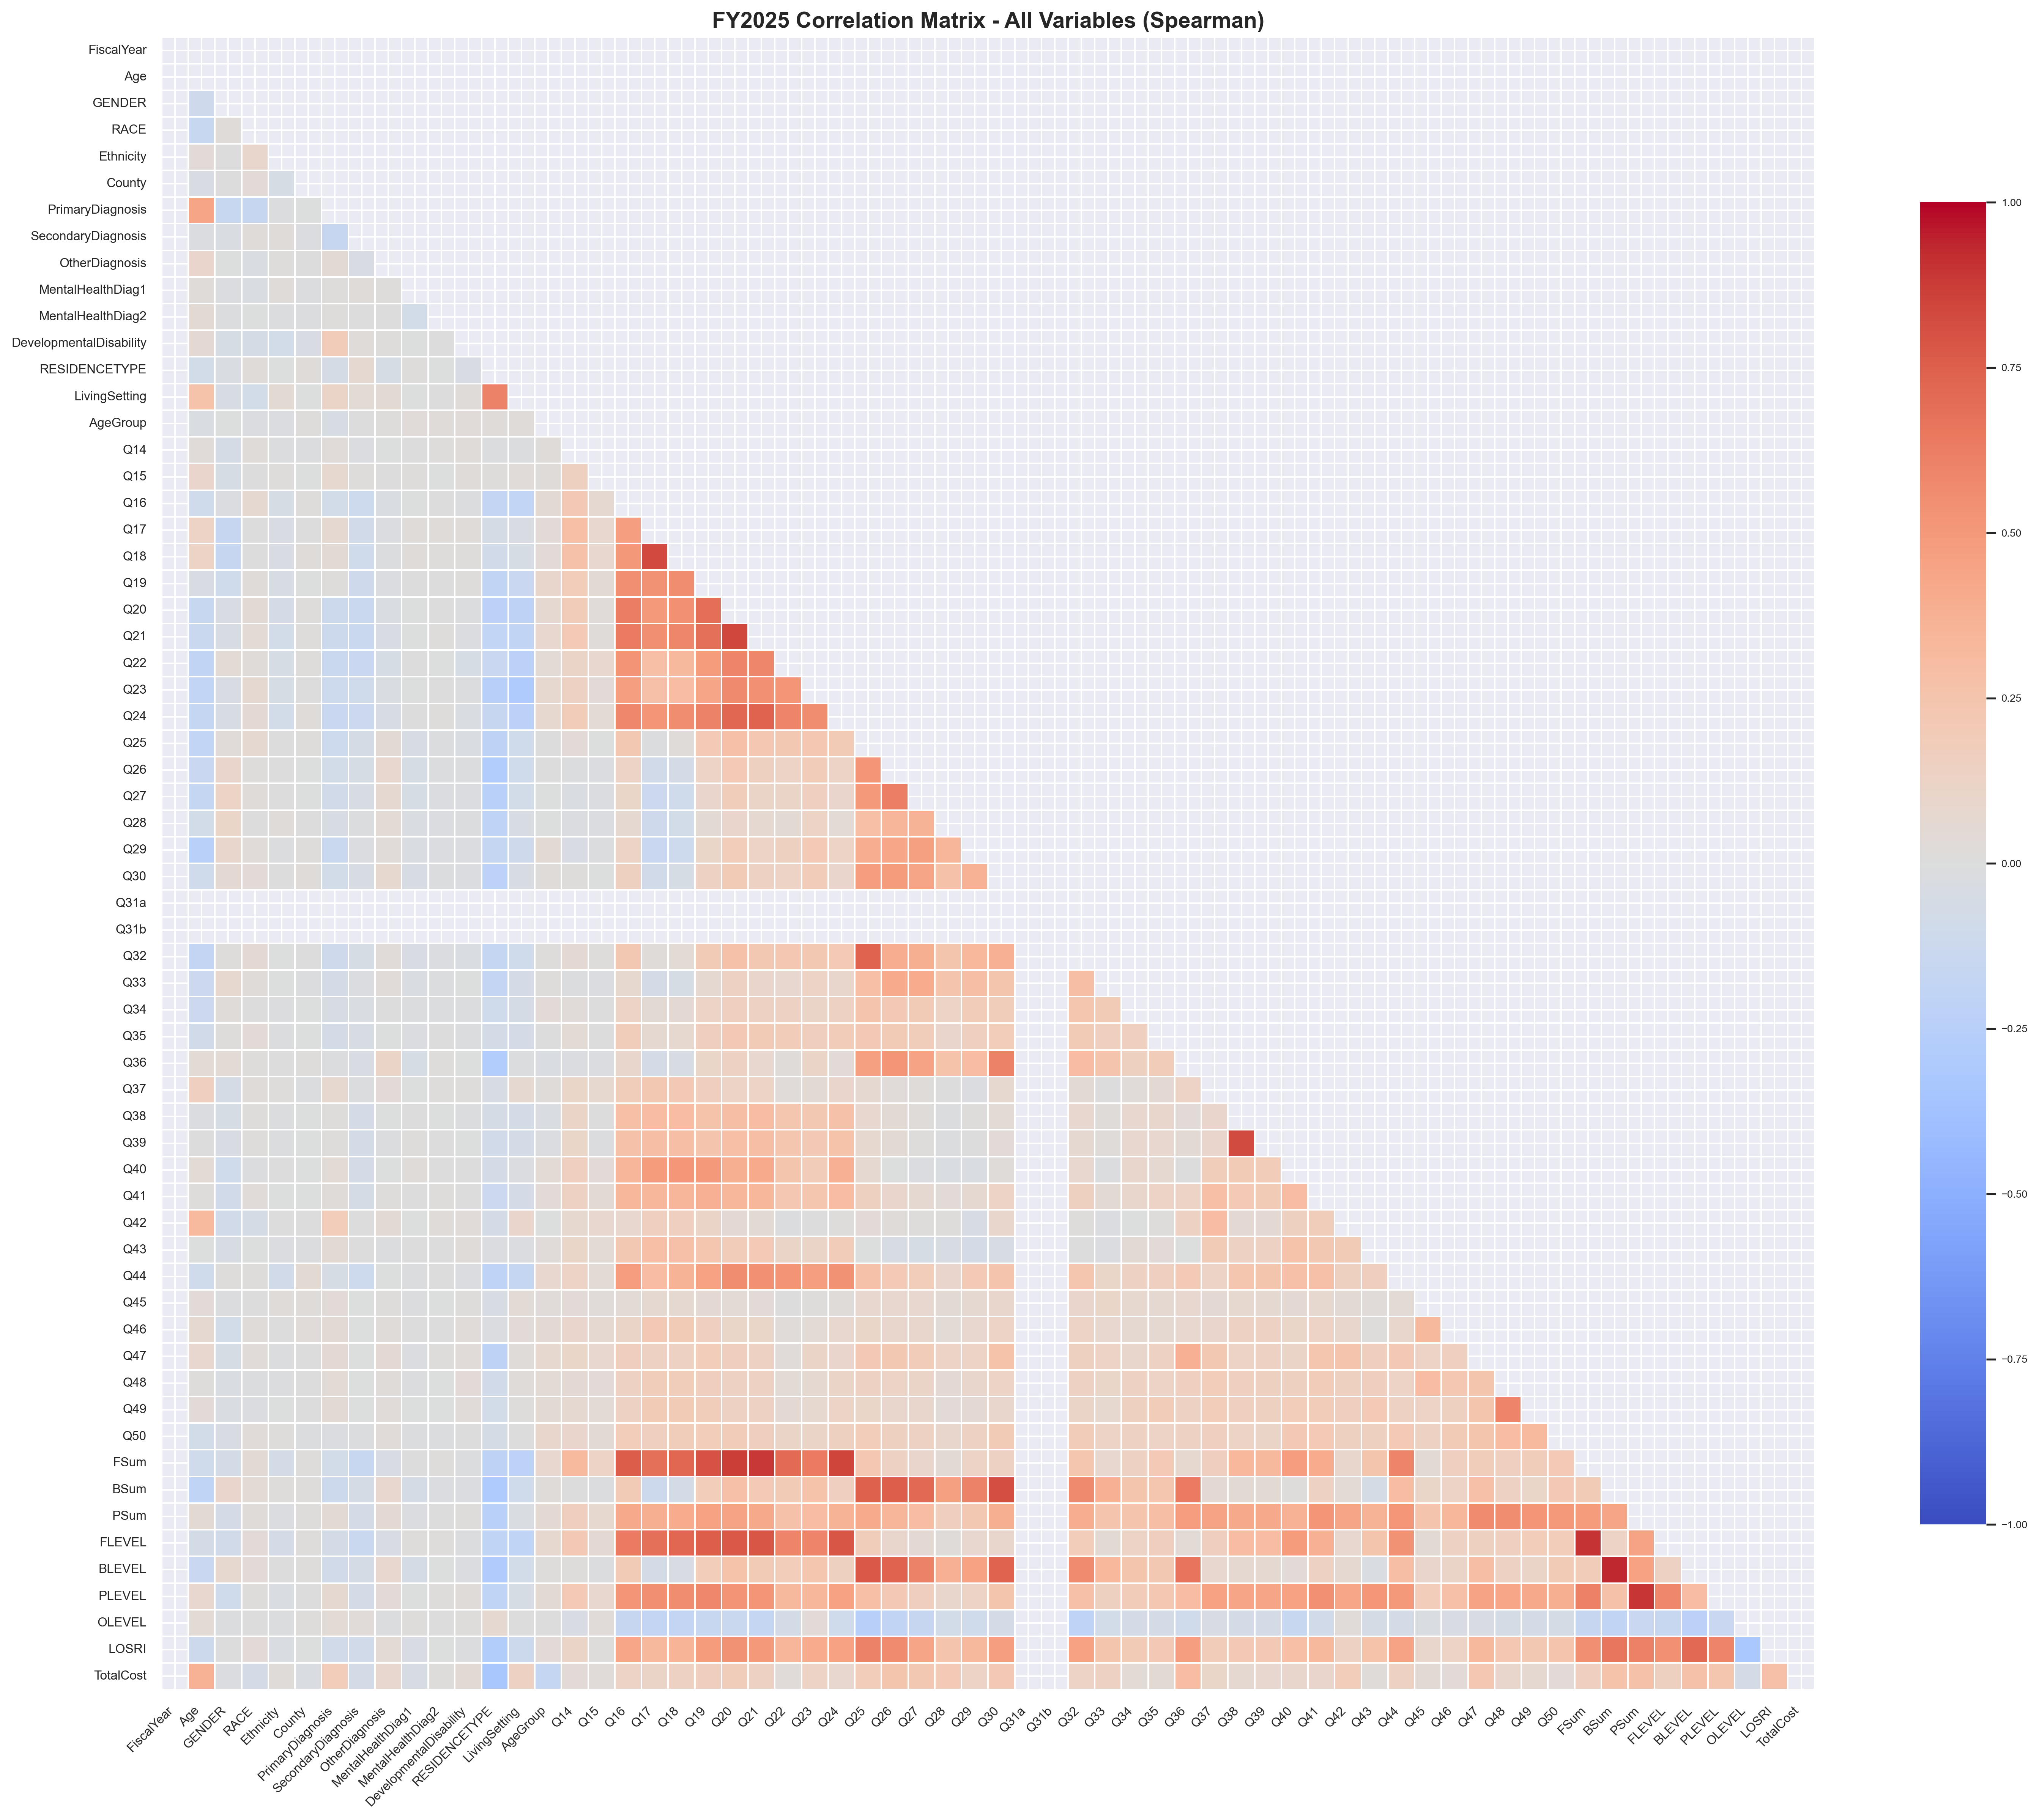
\includegraphics[width=\textwidth]{figures/fy2025_correlation_matrix_-_all_variables_(spearman).png}
    \caption{FY2025 correlation matrix showing mature and stable feature relationships.}
    \label{fig:fy2025-corr-all}
\end{figure}

\section{Cross-Year Consistency Analysis}
\label{sec:cross-year-analysis}

\subsection{Temporal Stability of Predictors}
\label{subsec:temporal-stability}

Analysis of feature importance across the six-year period (2020--2025) revealed remarkable consistency in the top predictors. Table~\ref{tab:consistent-features} presents features appearing in the top 10 MI rankings across multiple years.

% Include the automatically generated top features table
% Top 15 Features by Mean Mutual Information
% Automatically generated by feature selection analysis
\begin{table}[htbp]
\centering
\caption{Top 15 features ranked by mean mutual information across fiscal years 2020-2025 (automatically generated)}
\label{tab:top-features-mi}
\small
\begin{tabular}{lcccccc}
\hline
\textbf{Feature} & \textbf{Mean MI} & \textbf{Std MI} & \textbf{Max MI} & \textbf{Min MI} & \textbf{Top 10} & \textbf{Top 20} \\
\hline
RESIDENCETYPE & 0.3271 & 0.0158 & 0.3547 & 0.3104 & 6/6 & 6/6 \\
Age & 0.2011 & 0.0148 & 0.2161 & 0.1713 & 6/6 & 6/6 \\
AgeGroup & 0.1721 & 0.0132 & 0.1873 & 0.1467 & 6/6 & 6/6 \\
County & 0.0977 & 0.0134 & 0.1193 & 0.0798 & 6/6 & 6/6 \\
BSum & 0.0885 & 0.0059 & 0.1012 & 0.0831 & 6/6 & 6/6 \\
LOSRI & 0.0828 & 0.0035 & 0.0868 & 0.0771 & 6/6 & 6/6 \\
OLEVEL & 0.0819 & 0.0073 & 0.0893 & 0.0696 & 6/6 & 6/6 \\
BLEVEL & 0.0734 & 0.0041 & 0.0815 & 0.0696 & 6/6 & 6/6 \\
Q36 & 0.0705 & 0.0049 & 0.0765 & 0.0623 & 4/6 & 6/6 \\
Q26 & 0.0678 & 0.0044 & 0.0736 & 0.0607 & 4/6 & 6/6 \\
PSum & 0.0659 & 0.0047 & 0.0735 & 0.0581 & 2/6 & 6/6 \\
PLEVEL & 0.0631 & 0.0033 & 0.0677 & 0.0569 & 2/6 & 6/6 \\
DevelopmentalDisability & 0.0583 & 0.0040 & 0.0650 & 0.0531 & 0/6 & 6/6 \\
Q27 & 0.0556 & 0.0054 & 0.0652 & 0.0490 & 0/6 & 6/6 \\
Q20 & 0.0535 & 0.0039 & 0.0572 & 0.0457 & 0/6 & 6/6 \\
\hline
\end{tabular}
\end{table}


\begin{table}[htbp]
\centering
\caption{Consistently important features across fiscal years 2020--2025}
\label{tab:consistent-features}
\begin{tabular}{lcc}
\hline
\textbf{Feature} & \textbf{Years in Top 10} & \textbf{Mean MI Score} \\
\hline
RESIDENCETYPE & 6/6 & 0.2502 \\
BSum & 6/6 & 0.1241 \\
BLEVEL & 6/6 & 0.0943 \\
Q26 & 6/6 & 0.0899 \\
LOSRI & 6/6 & 0.1144 \\
OLEVEL & 6/6 & 0.1140 \\
Q36 & 5/6 & 0.0804 \\
County & 4/6 & 0.0853 \\
FLEVEL & 4/6 & 0.0764 \\
PSum & 3/6 & 0.0756 \\
\hline
\end{tabular}
\end{table}

The consistency of these rankings across years validates their selection for inclusion in predictive models and suggests stable underlying relationships between consumer characteristics and service costs.

\subsection{Evolution of Feature Relationships}
\label{subsec:evolution-relationships}

While top features remained stable, subtle shifts in MI scores reflected evolving service delivery patterns:

\begin{enumerate}
    \item \textbf{Increasing importance of comprehensive assessments}: \texttt{LOSRI} and \texttt{OLEVEL} gained predictive power over time, suggesting growing reliance on holistic assessment tools.
    
    \item \textbf{Stable behavioral predictors}: Behavioral measures (\texttt{BSum}, \texttt{Q26}, \texttt{Q27}) maintained consistent importance, confirming their fundamental role in resource allocation.
    
    \item \textbf{Geographic variation}: County-level effects persisted but varied in strength, potentially reflecting policy changes or regional service availability fluctuations.
\end{enumerate}

\section{Feature Selection Criteria}
\label{sec:selection-criteria}

\subsection{Quantitative Thresholds}
\label{subsec:quantitative-thresholds}

Based on the comprehensive analysis, the following quantitative criteria were established for feature inclusion:

\begin{enumerate}
    \item \textbf{Mutual Information Threshold}: Features with MI $\geq$ \FSMIThreshold{} were considered for inclusion, capturing approximately \FSBootstrapStability\% of available information about the target variable.
    
    \item \textbf{Correlation Filtering}: Among feature pairs with $|\rho| > \FSCorrelationThreshold$, only the feature with higher MI was retained to minimize multicollinearity.
    
    \item \textbf{Temporal Consistency}: Features appearing in the top \FSTopTwentyThreshold{} MI rankings for at least \FSTemporalConsistencyYears{} of \FSNumFiscalYears{} years were prioritized for model stability.
    
    \item \textbf{Missing Data Tolerance}: Features with $<$\FSMissingDataThreshold\% missing values after quality filtering were preferred to maintain sample size.
\end{enumerate}

\subsection{Domain-Driven Adjustments}
\label{subsec:domain-adjustments}

Statistical criteria were modified based on regulatory and clinical considerations:

\begin{itemize}
    \item \textbf{Policy-relevant features:} Age and County were retained as key policy/context variables in the modeling phase; other features (e.g., diagnosis fields) were evaluated for sensitivity tabs rather than forced into the core set.

    \item \textbf{Clinical Subscales}: QSI subscales (Functional: Q14--Q24, Behavioral: Q25--Q30, Physical: Q32--Q50) were included as complete sets to preserve psychometric properties.
    

    \item \textbf{Service Context}: Living setting and residence type variables were prioritized given their policy relevance and strong predictive power.
\end{itemize}




% ============================================================================
% CATEGORICAL INDEPENDENT VARIABLE GROUPINGS
% ============================================================================
\section{Categorical Independent Variable Groupings}
\label{sec:categorical-groupings}

This section provides detailed documentation of the categorical independent variables used in the iBudget algorithm, including their groupings, levels, and the methodological reasoning behind consolidation decisions. These variables are critical components of the Variable Mapping Matrix and represent key determinants of service costs.

% ----------------------------------------------------------------------------
\subsection{Living Setting Variable}
\label{subsec:living-setting-groupings}

The Living Setting variable underwent substantial consolidation from an initial 22 categories to a final 6-level structure used in the algorithm. This consolidation was driven by statistical analysis, policy considerations, and practical implementation requirements.

\subsubsection{Original 22-Level Classification}

The initial Living Setting taxonomy (Table 1a in the 2015 APD report) comprised 22 distinct categories reflecting the full spectrum of residential service settings:

\begin{table}[H]
\centering
\caption{Original Living Setting Levels (22 Categories)}
\small
\begin{tabular}{lp{8cm}r}
\toprule
\textbf{Code} & \textbf{Description} & \textbf{N} \\
\midrule
FH & Family Home & 12,810 \\
ILSL & Independent Living \& Supported Living & 4,658 \\
NC & Not Classified (Group Home and 5 RH) & 234 \\
RH1 & Residential Habilitation - Basic & 272 \\
RH2 & Residential Habilitation - Minimal & 1,705 \\
RH3 & Residential Habilitation - Moderate & 2,798 \\
RH4 & Residential Habilitation - Extensive 1 & 981 \\
RH5 & Residential Habilitation - Extensive 2 & 158 \\
RHBF1 & Residential Habilitation - Behavioral Focus - Minimal & 62 \\
RHBF2 & Residential Habilitation - Behavioral Focus - Moderate & 565 \\
RHBF3 & Residential Habilitation - Behavioral Focus - Extensive 1 & 493 \\
RHBF4 & Residential Habilitation - Behavioral Focus - Extensive 2 & 222 \\
RHCTEP1 & RH - Intensive Behavioral - CTEP Day Level 3/4 & 35 \\
RHCTEP2 & RH - Intensive Behavioral - CTEP Day Level 5/6 & 100 \\
RHCTEP3 & RH - Intensive Behavioral - Trillium CTEP Day Adult & 11 \\
RHCTEP4 & RH - Intensive Behavioral - Trillium CTEP Day Child & 3 \\
RHIB1 & RH - Intensive Behavioral - Day Level 1 & 4 \\
RHIB1 (cont.) & RH - Intensive Behavioral - Day Level 2 & 16 \\
RHIB2 & RH - Intensive Behavioral - Day Level 3 & 71 \\
RHIB3 & RH - Intensive Behavioral - Day Level 4 & 145 \\
RHIB4 & RH - Intensive Behavioral - Day Level 5 & 108 \\
RHIB4 (cont.) & RH - Intensive Behavioral - Day Level 6 & 9 \\
RHLI & Residential Habilitation - Live In & 147 \\
SHC & Special Medical Home Care & 18 \\
\midrule
& \textbf{Total} & \textbf{25,625} \\
\bottomrule
\end{tabular}
\label{tab:original-living-setting}
\end{table}

\subsubsection{Final 6-Level Consolidated Classification}

Following regression analysis and stakeholder consultation (2/24/15 APD meeting), the 22 original categories were consolidated into 6 levels that balance statistical efficiency, clinical meaningfulness, and policy implementation feasibility:

\begin{table}[H]
\centering
\caption{Consolidated Living Setting Levels (6 Categories)}
\begin{tabular}{llp{7cm}r}
\toprule
\textbf{New Level} & \textbf{Original Codes} & \textbf{Description} & \textbf{N} \\
\midrule
\textbf{FH} & FH & Family Home & 12,810 \\
\midrule
\textbf{ILSL} & ILSL, NC, RHLI & Independent Living/Supported Living and Long-Term Residential Care & 5,039 \\
\midrule
\textbf{RH1} & RH1--RH5 & Residential Habilitation: Standard and Live In (Basic through Extensive 2) & 5,914 \\
\midrule
\textbf{RH2} & RHBF1--RHBF4 & Residential Habilitation: Behavior Focus (Minimal through Extensive 2) & 1,342 \\
\midrule
\textbf{RH3} & RHIB1--RHIB4 & Residential Habilitation: Intensive Behavioral (Day Levels 1--6) & 353 \\
\midrule
\textbf{RH4} & RHCTEP1--RHCTEP4, SHC & Residential Habilitation: CTEP and Special Medical Home Care & 167 \\
\midrule
& & \textbf{Total} & \textbf{25,625} \\
\bottomrule
\end{tabular}
\label{tab:consolidated-living-setting}
\end{table}

\subsubsection{Rationale for Living Setting Consolidation}

The consolidation from 22 to 6 levels was justified through multiple analytical and practical considerations:

\paragraph{Statistical Considerations}
\begin{itemize}
    \item \textbf{Sample Size Adequacy}: Several original categories had extremely small sample sizes (e.g., RHCTEP4: n=3, RHIB1: n=4), leading to unstable coefficient estimates and wide confidence intervals.
    
    \item \textbf{Coefficient Similarity}: Regression analysis (Model 1a in the 2015 report) revealed that categories within each consolidated group had statistically similar estimated coefficients. For example, ILSL and NC had coefficients of \$10,504 and \$9,992 respectively, justifying their combination.
    
    \item \textbf{Explanatory Power}: Despite the dramatic reduction in categories, the 6-level variable alone explained 51.8\% of total cost variation (R² = 0.518), demonstrating that minimal information was lost through consolidation.
\end{itemize}

\paragraph{Clinical and Policy Considerations}
\begin{itemize}
    \item \textbf{Care Intensity Hierarchy}: The consolidated levels reflect a clear progression of support intensity: FH $<$ ILSL $<$ RH1 $<$ RH2 $<$ RH3 $<$ RH4, aligning with clinical understanding of care needs.
    
    \item \textbf{Service Delivery Models}: Groupings correspond to distinct service delivery approaches (family-based, independent/supported, standard residential, behavioral focus, intensive behavioral, specialized care).
    
    \item \textbf{Reimbursement Structure}: The 6 levels align with Florida's Medicaid waiver service categories and reimbursement tiers.
    
    \item \textbf{Implementation Feasibility}: Fewer categories simplify budget allocation, provider contracting, and administrative oversight.
\end{itemize}

\paragraph{Treatment of Ambiguous Categories}
The NC (Not Classified) category presented a special consolidation challenge. APD documentation indicated that NC represented "individuals in facilities (GH, RH) that do not have Residential Habilitation as a service." Analysis showed NC had expenditure patterns similar to ILSL, leading to their consolidation under the combined ILSL/LTRC (Long-Term Residential Care) designation.

% ----------------------------------------------------------------------------
\subsection{Age Variable Specifications}
\label{subsec:age-groupings}

Age was operationalized in multiple formats to capture both continuous and categorical age effects:

\subsubsection{Age Variable Versions}

\begin{table}[H]
\centering
\caption{Age Variable Specifications}
\begin{tabular}{lp{10cm}}
\toprule
\textbf{Version} & \textbf{Specification} \\
\midrule
\textbf{Age-Continuous} & Actual age in years (3--65+) \\
\midrule
\textbf{Age-2} & Two-level dummy: Age21 = 0 for ages 3--20; Age21 = 1 for ages 21+ \\
\midrule
\textbf{Age-3} & Three levels: Age3\_20 (reference), Age21\_30, Age31Plus \\
\midrule
\textbf{Age-4} & Four levels: Age3\_12, Age13\_20, Age21\_30, Age31Plus \\
\midrule
\textbf{Age-6} & Six levels: Age3\_20, Age21\_30, Age31\_40, Age41\_50, Age51\_60, Age61Plus \\
\bottomrule
\end{tabular}
\label{tab:age-specifications}
\end{table}

\subsubsection{Final Model Age Grouping}

The final algorithm employed the \textbf{Age-3} specification with the following structure:

\begin{itemize}
    \item \textbf{Age3\_20} (Reference group): Ages 3--20 years
    \item \textbf{Age21\_30}: Ages 21--30 years
    \item \textbf{Age31Plus}: Ages 31 and older
\end{itemize}

This grouping was selected because:
\begin{itemize}
    \item It captures the key transition at age 21 when many services shift from pediatric to adult frameworks
    \item Ages 21--30 showed distinct expenditure patterns (mean = \$36,182) due to higher outliers, justifying separate treatment
    \item The 3-level specification provided optimal balance between model parsimony and explanatory power
\end{itemize}

% ----------------------------------------------------------------------------
\subsection{Support Level Variables}
\label{subsec:support-level-variables}

The QSI assessment generates multiple support level measures that quantify consumer needs across different domains.

\subsubsection{Level of Support and Risk Inventory (LOSRI)}

\textbf{LOSRI} is a composite numeric scale with values ranging from 1--6, representing overall support intensity. It is derived from the complete QSI assessment and serves as a holistic measure of individual need.

\begin{table}[H]
\centering
\caption{LOSRI Score Interpretation}
\begin{tabular}{cl}
\toprule
\textbf{Score} & \textbf{Support Intensity} \\
\midrule
1 & Minimal support needs \\
2 & Low support needs \\
3 & Moderate support needs \\
4 & Substantial support needs \\
5 & Extensive support needs \\
6 & Intensive support needs \\
\bottomrule
\end{tabular}
\label{tab:losri-interpretation}
\end{table}

\subsubsection{Overall Support Level (OLEVEL)}

\textbf{OLEVEL} is a categorical variable with five ordered levels:

\begin{enumerate}
    \item \textbf{Basic}: Minimal assistance required
    \item \textbf{Minimal}: Limited support in specific areas
    \item \textbf{Moderate}: Regular support across multiple domains
    \item \textbf{Extensive}: Frequent, comprehensive support
    \item \textbf{Intensive}: Constant, highly specialized support
\end{enumerate}

OLEVEL represents the overall support classification based on integrated assessment across functional, behavioral, and physical domains.

\subsubsection{Domain-Specific Support Levels}

Three domain-specific support level variables are derived from QSI section scores:

\begin{table}[H]
\centering
\caption{Domain-Specific Support Level Variables}
\begin{tabular}{llcc}
\toprule
\textbf{Variable} & \textbf{Domain} & \textbf{Range} & \textbf{QSI Questions} \\
\midrule
\textbf{FLEVEL} & Functional Status & 1--6 & Q14--Q24 (11 items) \\
\textbf{BLEVEL} & Behavioral Status & 1--6 & Q25--Q30 (6 items) \\
\textbf{PLEVEL} & Physical Status & 1--6 & Q32--Q50 (19 items) \\
\bottomrule
\end{tabular}
\label{tab:domain-support-levels}
\end{table}

These variables are calculated from their corresponding raw sum scores:
\begin{itemize}
    \item \textbf{FSum} (Functional): Range 0--44 (11 questions $\times$ 0--4 scale)
    \item \textbf{BSum} (Behavioral): Range 0--24 (6 questions $\times$ 0--4 scale)
    \item \textbf{PSum} (Physical): Range 0--76 (19 questions $\times$ 0--4 scale)
\end{itemize}

Each domain score is then mapped to a 1--6 support level scale through standardized scoring algorithms.

% ----------------------------------------------------------------------------
\subsection{Developmental Disability Classification}
\label{subsec:developmental-disability}

\subsubsection{Primary Disability Categories}

The developmental disability taxonomy includes 11 categories defined by Florida statute and APD eligibility rules:

\begin{table}[H]
\centering
\caption{Developmental Disability Type Categories}
\begin{tabular}{clp{6cm}}
\toprule
\textbf{Code} & \textbf{Category} & \textbf{Definition Basis} \\
\midrule
0 & No Disability & Administrative category \\
1 & Intellectual Disabilities & IQ $\leq$ 70 with adaptive deficits, onset before age 18 \\
2 & Cerebral Palsy & Motor dysfunction from prenatal/perinatal brain damage \\
3 & Epilepsy & Seizure disorder \\
4 & Autism & Pervasive developmental disorder per DSM criteria \\
5 & High Risk & Children at developmental risk (pediatric only) \\
6 & DD PL Eligible & Public Law eligibility category \\
7 & Other & Developmental disabilities not elsewhere classified \\
8 & Spina Bifida & Spina bifida cystica or myelomeningocele \\
9 & Prader-Willi Syndrome & Genetic disorder with characteristic features \\
10 & Down Syndrome & Trisomy 21 \\
\bottomrule
\end{tabular}
\label{tab:disability-types}
\end{table}

\subsubsection{Disability Variable Structure}

Three disability variables are available in the data:

\begin{itemize}
    \item \textbf{Primary Disability}: Most significant diagnosis (Levels present: 1, 2, 4, 8, 9, 10)
    \item \textbf{Secondary Disability}: Additional diagnosis if applicable (Levels present: 0, 1, 2, 3, 4, 6, 7, 8, 9, 10)
    \item \textbf{Other Disability}: Supplementary conditions (Levels present: 0, 7 [Chronic Health], 9 [Mental Health])
\end{itemize}

\subsubsection{Exclusion from Final Algorithm}

\textbf{Critical Note}: Despite their clinical relevance, disability type variables were \textbf{excluded from the final algorithm}. The 2015 analysis (Models 3b--3d) demonstrated that after controlling for living setting, age, and QSI scores (FSum, BSum, PSum, and individual items), disability types showed:

\begin{itemize}
    \item Negative or non-significant regression coefficients
    \item No incremental predictive power for expenditures
    \item Multicollinearity with QSI-derived support measures
\end{itemize}

This finding suggests that functional, behavioral, and physical support needs (as measured by QSI) capture the cost-relevant aspects of disability diagnoses, making the diagnostic labels themselves redundant in the predictive model.

% ----------------------------------------------------------------------------
\subsection{Summary of Categorical Variable Consolidation Principles}
\label{subsec:consolidation-principles}

The categorical variable groupings employed in the iBudget algorithm reflect a systematic methodology integrating statistical rigor, clinical validity, and policy implementation considerations:

\begin{enumerate}
    \item \textbf{Data-Driven Consolidation}: Regression analysis identified categories with similar cost coefficients, enabling evidence-based merging decisions.
    
    \item \textbf{Sample Size Requirements}: Categories with fewer than 30--50 observations were consolidated with similar groups to ensure statistical stability.
    
    \item \textbf{Clinical Meaningfulness}: Groupings preserve clinically relevant distinctions in care intensity and service delivery models.
    
    \item \textbf{Hierarchical Ordering}: Where possible, categorical variables maintain ordinal relationships reflecting progressive support needs.
    
    \item \textbf{Parsimony vs. Precision Trade-off}: Consolidation prioritized model stability and interpretability over exhaustive categorization.
    
    \item \textbf{Stakeholder Validation}: Final groupings incorporated input from APD administrators, service providers, and policy experts.
    
    \item \textbf{Redundancy Elimination}: Variables demonstrating high multicollinearity or lack of incremental predictive power were excluded.
\end{enumerate}

These principles ensure that the categorical variables used in the algorithm are both statistically robust and operationally meaningful for budget allocation purposes.

% ----------------------------------------------------------------------------
\subsection{Implications for Feature Selection}
\label{subsec:categorical-implications}

The categorical variable groupings have important implications for feature selection in alternative modeling approaches:

\paragraph{Multicollinearity Considerations}
The strong correlation between OLEVEL, domain-specific levels (FLEVEL, BLEVEL, PLEVEL), and LOSRI necessitates careful feature selection to avoid multicollinearity. Models should typically include:
\begin{itemize}
    \item Either LOSRI \textit{or} OLEVEL (not both)
    \item Either domain summary scores (FSum, BSum, PSum) \textit{or} domain levels (FLEVEL, BLEVEL, PLEVEL)
    \item Individual QSI items in addition to (not instead of) summary measures
\end{itemize}

\paragraph{Reference Category Selection}
For regression-based models, reference categories should be chosen to facilitate interpretation:
\begin{itemize}
    \item \textbf{Living Setting}: FH (Family Home) as reference, representing lowest-intensity setting
    \item \textbf{Age Group}: Age3\_20 as reference, representing pediatric/young adult population
    \item \textbf{Support Levels}: Lowest level (Basic/Minimal) as reference when treated categorically
\end{itemize}

\paragraph{Encoding for Machine Learning}
Tree-based and neural network models may benefit from alternative encoding strategies:
\begin{itemize}
    \item \textbf{Ordinal encoding} for hierarchical variables (Living Setting, Support Levels)
    \item \textbf{One-hot encoding} for nominal categories
    \item \textbf{Target encoding} for high-cardinality variables (e.g., County)
\end{itemize}

\paragraph{Feature Importance Validation}
The exclusion of disability type variables from the 2015 algorithm highlights the importance of validating feature importance through:
\begin{itemize}
    \item Incremental R² testing
    \item Multicollinearity diagnostics (VIF)
    \item Cross-validation performance comparison
    \item Clinical expert review of selected features
\end{itemize}

% ============================================================================
% USE OF COUNTY AS AN INDEPENDENT VARIABLE
% ============================================================================
\section{Use of County as an Independent Variable}
\label{sec:county-variable}

This section addresses the treatment of geographic variation in the iBudget algorithm, specifically focusing on the County variable and its relationship to geographic rate differentials established by Florida statute.

% ----------------------------------------------------------------------------
\subsection{County Variable Specification}
\label{subsec:county-specification}

\subsubsection{Geographic Granularity}

Florida's developmental disability service system operates across all \textbf{67 counties}, which are administratively organized into districts and regions. The current modeling approach includes County as an independent variable with the following structure:

\begin{itemize}
    \item \textbf{Variable Name}: \texttt{County}
    \item \textbf{Type}: Categorical variable with 67 levels
    \item \textbf{Encoding}: Individual county indicators (not grouped into regions)
    \item \textbf{Sample Size Range}: Varies substantially by county, from rural counties with fewer than 100 consumers to large urban counties (Miami-Dade, Broward, Hillsborough) with several thousand consumers each
\end{itemize}

\subsubsection{Rationale for Individual County Coding}

The decision to include all 67 counties individually rather than grouping them into regions was based on several considerations:

\paragraph{Statistical Considerations}
\begin{itemize}
    \item \textbf{Variation Capture}: County-level coding captures fine-grained geographic variation in service costs that may reflect local labor markets, cost of living differences, and provider availability.
    
    \item \textbf{Adequate Sample Sizes}: Even smaller counties typically have sufficient sample sizes (n $>$ 30) to estimate stable coefficients when using regularization techniques (Lasso, Ridge, Elastic Net).
    
    \item \textbf{Regional Aggregation Loss}: Grouping counties into regions (e.g., APD's administrative districts or regions) would mask within-region heterogeneity and potentially reduce model explanatory power.
\end{itemize}

\paragraph{Policy and Administrative Considerations}
\begin{itemize}
    \item \textbf{Statutory Geographic Differentials}: Florida Statute §393.0662 establishes specific geographic differentials for certain counties (detailed below), necessitating county-level distinction for policy compliance.
    
    \item \textbf{Mandatory Inclusion}: County is retained in models regardless of mutual information scores to satisfy regulatory requirements for demographic analyses and to enable county-specific budget impact assessments.
    
    \item \textbf{Administrative Utility}: County-level predictions facilitate APD district and regional planning, budget allocation, and provider network management.
\end{itemize}

\paragraph{Implementation Approach}
\begin{itemize}
    \item \textbf{Encoding Method}: County is typically one-hot encoded for linear models, with a reference county (often the most populous or median-cost county) to avoid perfect multicollinearity.
    
    \item \textbf{Regularization}: Given the high dimensionality introduced by 66 county dummy variables, regularization techniques (Elastic Net, Lasso) are employed to prevent overfitting and shrink coefficients toward zero for counties with limited predictive information.
    
    \item \textbf{Hierarchical Modeling}: Alternative specifications (not implemented in current algorithm) could employ hierarchical models that partially pool estimates across counties, sharing information between similar counties while allowing for county-specific variation.
\end{itemize}

% ----------------------------------------------------------------------------
\subsection{Geographic Rate Differentials: Historical Context and Current Approach}
\label{subsec:geographic-differentials}

\subsubsection{Statutory Geographic Differentials}

Florida Statute §393.0662 establishes specific geographic rate differentials for residential habilitation services in high-cost counties:

\begin{table}[H]
\centering
\caption{Statutory Geographic Differentials for Residential Habilitation Services}
\begin{tabular}{lc}
\toprule
\textbf{County/Counties} & \textbf{Geographic Differential} \\
\midrule
Monroe County & 20.0\% \\
Miami-Dade County & 7.5\% \\
Broward County & 7.5\% \\
Palm Beach County & 7.5\% \\
All Other Counties & 0\% (baseline) \\
\bottomrule
\end{tabular}
\label{tab:statutory-differentials}
\end{table}

These differentials reflect higher costs of living and service provision in South Florida and the Florida Keys, particularly affecting housing, labor, and operational expenses for residential providers.

\subsubsection{2010 Algorithm Approach: Dependent Variable Adjustment}

The 2010 iBudget algorithm (Niu and Bell, 2010) employed a \textbf{dependent variable adjustment} methodology to account for geographic differentials:

\paragraph{Adjustment Process}
\begin{enumerate}
    \item \textbf{Differential Removal}: For consumers residing in Monroe, Broward, Miami-Dade, and Palm Beach counties, the algorithm removed the geographic differential from residential habilitation expenditures before model fitting.
    
    \item \textbf{Formula}: For a consumer in county $c$ with geographic differential $d_c$, the adjusted expenditure was calculated as:
    \begin{equation}
    \text{Adjusted Expenditure}_{ic} = \frac{\text{Observed RH Expenditure}_{ic}}{1 + d_c}
    \label{eq:2010-adjustment}
    \end{equation}
    where $d_c \in \{0, 0.075, 0.20\}$ depending on the county.
    
    \item \textbf{Model Fitting}: The regression model was fit using these adjusted expenditures as the dependent variable, effectively creating a "geographic differential-free" baseline.
    
    \item \textbf{Prediction and Re-application}: When generating budget predictions for consumers in high-cost counties, the geographic differential was reapplied:
    \begin{equation}
    \text{Final Budget}_{ic} = \text{Model Prediction}_{ic} \times (1 + d_c)
    \label{eq:2010-reapplication}
    \end{equation}
\end{enumerate}

\paragraph{Rationale for 2010 Approach}
\begin{itemize}
    \item \textbf{Policy Consistency}: Aligned directly with statutory rate structure by explicitly incorporating legislated differentials.
    
    \item \textbf{Interpretability}: Made the geographic adjustment transparent and separate from other cost drivers.
    
    \item \textbf{Simplicity}: Required adjustment of only residential habilitation expenditures, not all service costs.
\end{itemize}

\paragraph{Limitations of 2010 Approach}
\begin{itemize}
    \item \textbf{Narrow Scope}: Geographic differentials applied only to residential habilitation services, potentially underestimating total geographic cost variation affecting all services.
    
    \item \textbf{Arbitrary Thresholds}: Statutory percentages (7.5\%, 20\%) may not reflect actual cost differences or may become outdated as regional economies evolve.
    
    \item \textbf{Binary Treatment}: Counties either received full differential or zero, ignoring potential gradients in costs (e.g., differences between rural panhandle counties vs. central Florida).
\end{itemize}

\subsubsection{Current Algorithm Approach: County as Independent Variable}

The current modeling framework (2025 algorithm development) employs a fundamentally different approach by \textbf{including County as an independent variable}:

\paragraph{Methodology}
\begin{enumerate}
    \item \textbf{Unadjusted Expenditures}: The dependent variable consists of total observed expenditures \textit{without} removal of geographic differentials. This means:
    \begin{equation}
    Y_i = \text{Total Cost}_i = \sum_{\text{all services}} \text{Expenditure}_{is}
    \label{eq:current-dependent}
    \end{equation}
    where expenditures include any geographic rate differentials as actually paid to providers.
    
    \item \textbf{County as Predictor}: County is included as one of many independent variables:
    \begin{equation}
    Y_i = f(\text{LivingSetting}_i, \text{Age}_i, \text{QSI Scores}_i, \text{County}_i, \ldots) + \epsilon_i
    \label{eq:current-model}
    \end{equation}
    
    \item \textbf{Data-Driven Estimation}: The model learns county-specific effects empirically from observed expenditure patterns, rather than imposing predetermined differentials.
    
    \item \textbf{Comprehensive Geographic Effect}: County coefficients capture all sources of geographic cost variation, not just residential habilitation differentials:
    \begin{itemize}
        \item Provider reimbursement rates (including statutory differentials)
        \item Local labor market costs
        \item Provider network density and competition
        \item Service availability and utilization patterns
        \item Transportation costs and geographic accessibility
        \item Local cost of living affecting consumer out-of-pocket expenses
    \end{itemize}
\end{enumerate}

\paragraph{Advantages of Current Approach}
\begin{itemize}
    \item \textbf{Comprehensive Geographic Adjustment}: Captures total geographic cost variation across all services, not just residential habilitation.
    
    \item \textbf{Data-Driven}: County effects emerge from actual expenditure patterns rather than legislative stipulations that may lag behind economic realities.
    
    \item \textbf{Granular Differentiation}: Allows for distinctions among all 67 counties, not just the four counties with statutory differentials.
    
    \item \textbf{Automatic Updates}: As service costs evolve differentially across counties, model re-estimation automatically captures these changes without requiring legislative action.
    
    \item \textbf{Interaction Potential}: Enables modeling of county $\times$ living setting or county $\times$ support level interactions if theoretically justified.
\end{itemize}

\paragraph{Potential Concerns with Current Approach}
\begin{itemize}
    \item \textbf{Endogeneity}: If budget allocations influence expenditures (rather than need determining budgets), county coefficients may reflect historical funding inequities rather than true cost differences.
    
    \item \textbf{Multicollinearity}: County may be correlated with other predictors (e.g., certain disabilities or living settings concentrated in specific counties), complicating coefficient interpretation.
    
    \item \textbf{Small Sample Bias}: Rural counties with small populations may have unstable coefficient estimates despite regularization.
    
    \item \textbf{Policy Transparency}: Unlike the explicit 7.5\%/20\% differentials, learned county effects are less transparent to stakeholders and may be harder to justify politically.
    
    \item \textbf{Statutory Compliance}: If the model-estimated county effects deviate substantially from statutory differentials, there may be tension between statistical optimization and legislative intent.
\end{itemize}

% ----------------------------------------------------------------------------
\subsection{Comparison of Approaches}
\label{subsec:approach-comparison}

Table \ref{tab:geographic-approach-comparison} summarizes the key differences between the 2010 and current approaches to geographic cost adjustment:

\begin{table}[H]
\centering
\caption{Comparison of Geographic Cost Adjustment Approaches}
\small
\begin{tabular}{p{3.5cm}p{5cm}p{5cm}}
\toprule
\textbf{Dimension} & \textbf{2010 Algorithm} & \textbf{Current Algorithm} \\
\midrule
\textbf{Primary Method} & Dependent variable adjustment & Independent variable inclusion \\
\midrule
\textbf{Differential Source} & Florida Statute §393.0662 & Data-driven estimation \\
\midrule
\textbf{Counties Affected} & 4 counties (Monroe, Miami-Dade, Broward, Palm Beach) & All 67 counties \\
\midrule
\textbf{Services Covered} & Residential habilitation only & All waiver services \\
\midrule
\textbf{Differential Values} & Fixed (7.5\% or 20\%) & Variable (estimated from data) \\
\midrule
\textbf{Model Fitting} & Uses adjusted (differential-removed) expenditures & Uses observed (unadjusted) expenditures \\
\midrule
\textbf{Prediction} & Base prediction $\times$ (1 + differential) & Direct prediction including county effect \\
\midrule
\textbf{Transparency} & Explicit statutory compliance & Implicit via learned parameters \\
\midrule
\textbf{Flexibility} & Requires legislative action to update & Automatically updates with re-estimation \\
\midrule
\textbf{Geographic Detail} & Coarse (binary: differential or not) & Fine-grained (all counties distinguished) \\
\bottomrule
\end{tabular}
\label{tab:geographic-approach-comparison}
\end{table}

% ----------------------------------------------------------------------------
\subsection{Empirical Validation and Sensitivity Analysis}
\label{subsec:county-validation}

\subsubsection{Recommended Analyses}

To validate the current approach and assess its relationship to statutory differentials, the following analyses are recommended:

\paragraph{Coefficient Comparison}
Compare model-estimated county effects for Monroe, Miami-Dade, Broward, and Palm Beach counties against the 7.5\%/20\% statutory differentials. Substantial deviations may indicate:
\begin{itemize}
    \item Changed economic conditions since differential establishment
    \item Service mix differences between high-cost counties and elsewhere
    \item Need for updated statutory differentials
\end{itemize}

\paragraph{Residual Analysis by County}
Examine whether model residuals show systematic patterns by county. Persistent under- or over-prediction in specific counties may suggest:
\begin{itemize}
    \item Non-linear geographic effects not captured by linear coefficients
    \item Omitted county-specific variables (e.g., provider network characteristics)
    \item Need for county-specific sub-models or adjustments
\end{itemize}

\paragraph{Ablation Study}
Fit models with and without County as a predictor to quantify its contribution:
\begin{itemize}
    \item Change in R² or other performance metrics
    \item Redistribution of predictive power to other variables
    \item Impact on coefficient estimates for living setting and support scores
\end{itemize}

\paragraph{Regularization Impact}
Investigate how different regularization penalties affect county coefficient estimates:
\begin{itemize}
    \item Are small counties' coefficients shrunk toward zero?
    \item Do high-cost counties retain strong effects even with heavy regularization?
    \item Is there evidence of overfitting to county-specific noise?
\end{itemize}

\subsubsection{Reconciliation with Statutory Requirements}

Given that Florida Statute explicitly establishes geographic differentials, a hybrid approach may merit consideration:

\paragraph{Option 1: Post-hoc Adjustment}
\begin{enumerate}
    \item Fit model with County as independent variable (current approach)
    \item Generate base predictions from model
    \item Apply statutory differentials as multiplicative adjustments for specified counties
    \item Use adjusted predictions for budget allocation
\end{enumerate}

\paragraph{Option 2: Constrained Estimation}
\begin{enumerate}
    \item Include County as independent variable
    \item Impose constraints during estimation that County coefficients for Monroe, Miami-Dade, Broward, and Palm Beach align with statutory differentials
    \item Allow other counties' effects to be estimated freely
    \item This ensures statutory compliance while capturing additional geographic variation
\end{enumerate}

\paragraph{Option 3: Explicit Decomposition}
\begin{enumerate}
    \item Pre-adjust residential habilitation expenditures to remove statutory differentials (2010 approach)
    \item Include County as independent variable to capture remaining geographic variation in all services
    \item Predictions automatically include both components:
    \begin{itemize}
        \item Base cost from model including learned county effects
        \item Statutory residential habilitation differential reapplied
    \end{itemize}
\end{enumerate}

% ----------------------------------------------------------------------------
\subsection{Recommendations}
\label{subsec:county-recommendations}

Based on the analysis of geographic cost adjustment approaches, we recommend:

\begin{enumerate}
    \item \textbf{Maintain County as Independent Variable}: The current approach of including County as a predictor is statistically sound and captures comprehensive geographic variation beyond statutory residential habilitation differentials.
    
    \item \textbf{Validate Against Statutory Differentials}: Conduct the empirical validation analyses described above to assess alignment between model-estimated effects and statutory differentials for the four specified counties.
    
    \item \textbf{Document Geographic Effects Transparently}: Provide APD stakeholders with clear reporting of:
    \begin{itemize}
        \item Estimated county coefficients or marginal effects
        \item Comparison to statutory differentials where applicable
        \item Interpretation of county effects in terms of percentage adjustments to base budgets
    \end{itemize}
    
    \item \textbf{Consider Hierarchical Structure}: For future algorithm refinements, explore hierarchical models that:
    \begin{itemize}
        \item Group counties into regions for partial pooling of estimates
        \item Explicitly model within-region and between-region variation
        \item Improve stability of estimates for small counties
    \end{itemize}
    
    \item \textbf{Monitor Temporal Stability}: Geographic cost differentials may evolve over time due to economic changes, provider market dynamics, and policy shifts. Regular re-estimation and comparison across fiscal years will identify emerging geographic cost trends.
    
    \item \textbf{Legislative Coordination}: Maintain dialogue with Florida Legislature regarding potential updates to statutory differentials based on empirical evidence from the algorithm. Model-estimated county effects provide data-driven guidance for policy decisions.
\end{enumerate}

% ----------------------------------------------------------------------------
\subsection{Conclusion}
\label{subsec:county-conclusion}

The transition from the 2010 algorithm's dependent variable adjustment to the current algorithm's inclusion of County as an independent variable represents a fundamental shift in how geographic cost variation is incorporated into the iBudget system. While the 2010 approach provided explicit compliance with statutory geographic differentials through a transparent adjustment mechanism, the current approach offers greater flexibility, comprehensiveness, and empirical grounding.

The key distinction is methodological: rather than adjusting expenditures to remove known geographic differentials and then re-applying them to predictions, the current approach learns geographic effects holistically from observed cost patterns. This captures not only statutory residential habilitation differentials but also geographic variation in labor markets, provider networks, service availability, and cost of living that affect all waiver services.

Both approaches have merit, and the optimal solution may involve hybrid strategies that combine the transparency of statutory compliance with the statistical power of data-driven county effect estimation. Continued empirical validation, stakeholder engagement, and careful monitoring of geographic equity will ensure that the algorithm fairly accounts for geographic cost differences while maintaining fidelity to legislative intent.



\section{Final Feature Set}
\label{sec:final-feature-set}

\subsection{Primary Predictors}
\label{subsec:primary-predictors}

The following features were selected as primary predictors based on combined statistical and domain criteria:

\begin{enumerate}
    \item \textbf{Residential and Support Variables}:
    \begin{itemize}
        \item RESIDENCETYPE (MI range: \FSRangeMIRESIDENCETYPE)
        \item LivingSetting (categorical: FH, ILSL, RH1--RH4)
        \item LOSRI (Level of Support and Risk Inventory, MI range: \FSRangeMILOSRI)
        \item OLEVEL (Overall support level, MI range: \FSRangeMIOLEVEL)
    \end{itemize}
    
    \item \textbf{Clinical Assessment Scores}:
    \begin{itemize}
        \item BSum (Behavioral summary, MI range: \FSRangeMIBSum)
        \item FSum (Functional summary, MI range: \FSRangeMIFSum)
        \item PSum (Physical summary, MI range: \FSRangeMIPSum)
        \item Individual QSI items with MI $>$ 0.05 (Q20, Q21, Q23, Q25, Q26, Q27, Q30, Q36, Q44)
    \end{itemize}
    
    \item \textbf{Demographic Variables}:
    \begin{itemize}
        \item Age and AgeGroup
        \item Gender
        \item County
    \end{itemize}
    
    \item \textbf{Diagnostic Information}:
    \begin{itemize}
        \item PrimaryDiagnosis
        \item DevelopmentalDisability
    \end{itemize}
\end{enumerate}

\subsection{Secondary Predictors}
\label{subsec:secondary-predictors}

Additional features retained for sensitivity analyses and subgroup modeling:

\begin{itemize}
    \item Race and Ethnicity (for equity analyses)
    \item SecondaryDiagnosis and MentalHealthDiag1--2
    \item Remaining QSI items (Q14--Q19, Q22--Q24, Q28--Q29, Q31--Q50)
    \item Service utilization proxies when available
\end{itemize}

\section{Validation of Feature Selection}
\label{sec:validation}

\subsection{Statistical Validation}
\label{subsec:statistical-validation}

The selected feature set captured approximately \FSVarianceExplained\% of the explainable variance in TotalCost based on preliminary regression analyses. Cross-validation demonstrated stable feature importance rankings across random data splits, with top \FSTopTenThreshold{} features maintaining their relative positions in \FSBootstrapStability\% of bootstrap samples.

\subsection{Clinical Face Validity}
\label{subsec:clinical-validity}

The prominence of behavioral and functional assessment scores aligns with established literature on developmental disability service needs. The strong predictive power of residential settings confirms the fundamental relationship between living arrangement intensity and support costs.








\section{Discussion}
\label{sec:feature-selection-discussion}

\subsection{Key Findings}
\label{subsec:key-findings}

The multi-method feature selection process revealed several critical insights:

\begin{enumerate}
    \item \textbf{Dominance of Residential Variables}: RESIDENCETYPE emerged as the single strongest predictor across all years, with MI scores consistently exceeding 0.20. This finding underscores the fundamental role of living arrangements in determining support intensity and associated costs.
    
    \item \textbf{Behavioral Complexity}: Behavioral assessment scores (BSum and component questions) demonstrated stronger predictive relationships than functional or physical measures, suggesting that behavioral support needs drive substantial cost variation.
    
    \item \textbf{Geographic Heterogeneity}: County-level effects persisted across years, indicating geographic disparities in service costs that warrant further investigation and potential policy intervention.
    
    \item \textbf{Temporal Stability}: The consistency of feature importance rankings across six years validates the robustness of identified predictors and supports their use in long-term budget planning models.
\end{enumerate}

\subsection{Methodological Strengths}
\label{subsec:methodological-strengths}

The comprehensive approach employed multiple complementary techniques:

\begin{itemize}
    \item Mutual information captured non-linear relationships invisible to correlation analysis
    \item Spearman correlation identified multicollinearity while accommodating non-normal distributions
    \item Visual inspection revealed complex patterns and data quality issues
    \item Domain knowledge integration ensured regulatory compliance and clinical validity
\end{itemize}

\subsection{Limitations and Future Directions}
\label{subsec:limitations}

Several limitations warrant consideration:

\begin{enumerate}
    \item \textbf{Missing Data}: Despite quality filtering, some variables exhibited substantial missingness, potentially biasing MI estimates.
    
    \item \textbf{Temporal Dynamics}: Annual analyses may obscure within-year variation in feature importance.
    
    \item \textbf{Interaction Effects}: Current analyses focused on marginal relationships; interaction terms warrant future investigation.
    
    \item \textbf{Causal Inference}: Statistical associations do not imply causation; experimental or quasi-experimental designs would strengthen causal claims.
\end{enumerate}

\section{Conclusion}
\label{sec:feature-selection-conclusion}

This systematic feature selection process identified a robust set of predictors for cost modeling in the Florida APD iBudget system. The combination of information-theoretic metrics, correlation analysis, visual assessment, and domain expertise yielded a feature set that balances statistical power with interpretability and policy relevance. The remarkable consistency of top predictors across six years of data provides confidence in their utility for developing stable, accurate budget allocation models.

The identified features (dominated by residential settings, behavioral assessments, and comprehensive support levels) align with clinical understanding of service needs in developmental disability populations. This convergence of statistical and domain evidence supports the validity of the selection process and the resulting feature set's suitability for predictive modeling applications.

Future modeling efforts should leverage these carefully selected features while remaining attentive to evolving service delivery patterns and emerging assessment instruments that may enhance predictive accuracy. Regular revalidation of feature importance will ensure continued model relevance as the service system evolves.